\documentclass[a4paper,11pt]{article}

\usepackage[utf8]{inputenc}
\usepackage[czech]{babel}
\usepackage[left=2cm,top=3cm,text={17cm,24cm}]{geometry}
\usepackage{graphicx}
\usepackage{listings}
\usepackage{url}

\title{ISA - Síťové aplikace a správa sítí\\
{\bf\large Laboratorní manuál}}

\author{Vysoké učení technické v Brně}

\date{\url{https://github.com/nesfit/ISA/tree/master/manual}}

\begin{document}

{\let\newpage\relax\maketitle}

Tento laboratorní manuál slouží jako referenční příručka pro laboratorní cvičení
předmětu ISA -- Síťové aplikace a správa sítí. Očekává se, že si studenti před
účastí na jednotlivých cvičeních přečtou sekce potřebné pro dané cvičení.

Sekce \ref{adresy_ipv4}, \ref{adresy_ipv6}, \ref{basics}, \ref{wireshark} a \ref{ipconfig} jsou
potřebné pro všechny cvičení. Cvičení \emph{Zabezpečený přenos dat} navíc
předpokládá znalosti ze sekce~\ref{ntp}, \ref{ssh} a~\ref{tls}. Ve cvičení \emph{DNS,
DNSSEC} se využívají sekce \ref{dns} a \ref{dnssec}. Cvičení
\emph{Konfigurace a analýza přenosů VoIP} předpokládá znalosti uvedené v
sekci~\ref{sip}. Cvičení \emph{Správa a monitorování sítě} staví na informacích
uvedených v sekcích \ref{syslog} a \ref{netflow}.

\setcounter{tocdepth}{1}
\tableofcontents
\newpage

\section{Adresy v~IPv4 síti}\label{adresy_ipv4}

\subsection{Formát adresy}
IPv4 adresa je délky 32 bitů a preferovaný zápis má formát {\tt X.X.X.X}, kde
{\tt X} je decimální zápis 8 bitového čísla. Příklad:\\
\begin{verbatim}
8.8.8.8
127.0.0.1
\end{verbatim}

Adresa dvě části:
\begin{itemize}
    \item adresa sítě ({\bf prefix}) a
    \item adresa uzlu.
\end{itemize}
Délka prefixu se zapisuje v~desítkovém tvaru za lomítko. {\tt 192.168.0.1/24}

V~síti s~daným prefixem existují 2 speciální adresy, které nelze použít pro
adresování jednotlivých uzlů:
\begin{itemize}
    \item adresa sítě - adresa uzlu je nulová, např. 192.168.0.0/24
    \item broadcastová adresa - nejvyšší možná adresa uzlu pro daný prefix,
        např. 192.168.0.255/24
\end{itemize}

\section{Adresy v~IPv6 síti}\label{adresy_ipv6}

\subsection{Formát adresy}
IPv6 adresa je délky 128 bitů a zapsaných ve formátu {\tt X:X:X:X:X:X:X:X}, kde
{\tt X} je hexadecimální zápis 16 bitového čísla.
Příklad:\\
\begin{verbatim}
FEDC:BA98:7654:3210:fedc:ba98:7654:3210
1080:0000:0000:0000:0008:0800:200C:417a
\end{verbatim}

Preferovaný formát je dále upraven v~RFC 5952\footnote{https://tools.ietf.org/html/rfc5952}, které definuje následující
pravidla:
\begin{itemize}
    \item Nuly na začátku každého 16 bitového čísla je potřeba vynechat (např.
        80 namísto 0080 a 0 namísto 0000).
    \item Více nulových bloků lze nejvýše jednou nahradit znakem {\tt ::}, a
        MUSÍ být nahrazena nejdelší možná posloupnost takových nulových bloků.
        V~případě více shodně dlouhých posloupností, nahrazuje se ta nejvíce
        vlevo.
    \item Znak {\tt ::} nesmí nahrazovat samostatný nulový blok.
    \item Znaky "a", "b", "c", "d", "e", "f" hexadecimální soustavy se vždy
        píšou malými písmeny.
\end{itemize}
Adresy z~předchozího příkladu tedy budou vypadat následovně:\\
\begin{verbatim}
fedc:ba98:7654:3210:fedc:ba98:7654:3210
1080::8:800:200c:417a
\end{verbatim}

Stejně jako v~IPv4 má adresa dvě části: \emph{adresa sítě ({\bf prefix})} a
\emph{adresa uzlu}. Délká prefixu se zapisuje v~desítkovém tvaru za lomítko
(např. {\tt 1080::/60}).

\subsection{Rozdělení adres}
IPv6 adresy je možno rozdělit podle rozsahu. Typicky může jít o~tři
možnosti -- adresy na lince (neprojdou za router), lokální adresy (ULA, nejsou
routovatelné ve veřejné sítí) a veřejné adresy.

\begin{table}[ht!]
    \begin{center}
        \begin{tabular}{l|l|l}
            Význam & Prefix (bitově) & Prefix \\
            \hline\hline
            Veřejné  & {\tt 001} & {\tt 2000::/3} \\
            \hline
            Lokální  & {\tt 1111 110} & {\tt FC00::/7} \\
            \hline
            Linkové  & {\tt 1111 1110 10} & {\tt FE80::/10} \\
            \hline
            Multicast & {\tt 1111 1111} & {\tt FF00::/8} \\
            \hline
        \end{tabular}
    \end{center}
\end{table}

\subsection{Lokální IPv6 (ULA) adresy}\label{ula}

Tyto adresy jsou vhodné pro malé sítě zahrnující jedno místo, nebo organizaci.
Adresy ULA nejsou globálně směrovatelné (ale nic nebrání jedné, či více
organizacím své adresy mezi sebou směrovat). Jedním z využití adres ULA je
získání celosvětově unikátního prefix bez formálních požadavků na registraci
adres.

Síťová část ULA adresy se stává ze 4 části:
\begin{description}
    \item [Prefix] {\tt fc00::/7}
    \item [L] bit 1 pokud byl prefix přiřazen lokálně, 0 zatím nebyla
        definována, začátek adresy je proto typicky {\tt fd00::/8}
    \item [Global ID] identifikátor sítě, měl by být unikátní, standard
        popisuje pseudonáhodný algoritmus pro generování. Unikátnost je
        požadována, aby při spojení více lokálních sítí nebylo třeba žádnou
        přečíslovat.
    \item [Inderface ID] Identifikátor rozhraní, existuje několik variant jak
        jej získat. Původní standard (RFC
        3513\footnote{https://tools.ietf.org/html/rfc3513} a RFC
        4291\footnote{https://tools.ietf.org/html/rfc4291}) doporučoval použití
        EUI-64. V~současnosti byla tato metoda nahrazena RFC
        7217\footnote{https://tools.ietf.org/html/rfc7217}. Pro ochranu
        soukromí jsou další specifika automatické generace identifikátorů
        definovány v~RFC 4941\footnote{https://tools.ietf.org/html/rfc4941}.
\end{description}

\begin{table}[ht!]
    \begin{center}
        \begin{tabular}{c|c|c|c|c}
            7 bits & 1 &  40 bits  &  16 bits  & 64 bits \\
            \hline
            1111 110 & L & Global ID & Subnet ID & Interface ID \\
            \hline
        \end{tabular}
    \end{center}
\end{table}

Lokální síť je tedy složená ze tří části:
\begin{itemize}
    \item unikátní prefix délky 48 bitů,
    \item 16 bitový identifikátor podsítě,
    \item adresa uzlu o~délce 64 bitů.
\end{itemize}


%%%%%%%%%%%%%%%%%%%%%%%%%%%%%%%%%%%%%%
\section{Základy konfigurace linuxového serveru}
\label{basics}

Detailní popis včetně možných voleb a příkladu použití k~jednotlivým níže zmíněným příkazům můžete nalézt v~manuálových stránkách (\texttt{man <příkaz>}).
\subsection{Základní orientace v~Linuxu}
Většina práce v~OS Linux bude probíhat v~terminálu. Terminál na školních PC spustíte pomocí \texttt{Alt+F2}, zde zadáte "\texttt{gnome-terminal}". Případně můžete vybrat aplikaci terminálu z~postraní nabídky.
\subsubsection{Hierarchie souborového systému}
Všechny soubory jsou uloženy v~souborovém systému. Ten je organizován jako invertovaný strom adresářů,
kde kořenovým adresářem je \texttt{root} adresář (označení \texttt{"/"}). Ten obsahuje podadresáře,
kde každý má svůj standardizovaný účel pro zařazení různých souborů.

Některé podadresáře a jejich význam:
\begin{itemize}
				\item \textbf{/etc} - obsahuje konfigurační soubory systému,
				\item \textbf{/var} - proměnlivá boot perzistentní data, dynamicky se mění, obsahuje databáze, cache adresáře, obsah www stránek (\texttt{/var/html/www}), logy (\texttt{/var/log}),
				\item \textbf{/dev} - obsahuje speciální soubory pro přístup k~hardware zařízením.
\end{itemize}

\subsubsection{Základní příkazy}
Některé základní příkazy pro práci v~terminálu OS Linux:
\begin{itemize}
				\item \texttt{cd} - posun v~adresářové hierarchii,
				\item \texttt{ls} - zobrazení obsahu adresáře,
				\item \texttt{cp} - kopírování souborů,
				\item \texttt{mv} - přesun souborů,
				\item \texttt{mkdir} - vytvoření adresáře,
				\item \texttt{touch} - vytvoření prázdného souboru,
				\item \texttt{head} - zobrazení x řádků od začátku souboru,
				\item \texttt{tail} - zobrazení x řádků z~konce souboru,
				\item \texttt{cat} - zobrazení obsahu souboru,
				\item \texttt{grep} - filtrování/hledání v~textu,
				\item \texttt{sed} - editace textu v~příkazové řádce,
				\item \texttt{awk} - skenování a zpracování textu,
				\item \texttt{ps} - zobrazení informací o~běžících procesech.
\end{itemize}

Mezi command line editory patří například \texttt{nano} nebo \texttt{vim}. Kromě nich můžete taktéž použít grafické editory, například \texttt{gedit}.

\subsubsection{Uživatelé}
Každý uživatel v~OS Linux má své jedinečné \texttt{uid}. Každý proces (program)
v~systému je spuštěn pod nějakým uživatelem. Každý soubor je vlastněn uživatelem
a omezen přístupovými právy. Tato přístupová práva se vztahují taktéž na procesy
spuštěné daným uživatelem.

\begin{itemize}
				\item \texttt{root} - super uživatel, má veškerá práva a kontrolu nad systémem.
				\item \texttt{user} - pouze základní správa, bez možnosti zasahovat do systémového nastavení.
				\item \texttt{sudo} - delegace některých práv super uživatele na normálního uživatele (nastavení v~\texttt{/etc/sudoers}).
\end{itemize}

Při správě OS se pokud možno snažíme vyhnout používání systému jako \texttt{root}. K~tomuto slouží \texttt{sudo},
kde má daný uživatel přesně specifikováno, které operace smí se systémem provádět, a je pak lépe dohledatelné,
kdo co nastavil.

Přepínání uživatele:
\texttt{su [user]}
\begin{itemize}
				\item \texttt{su} - přepnutí na uživatele \texttt{root}.
				\item \texttt{su user} - přepnutí na uživatele \texttt{user}.
\end{itemize}

Spouštění příkazů jako \texttt{sudo}:
\texttt{sudo command...}

\subsection{Správa systémových služeb}
\label{sluzby}

OS Linux poskytuje řadu různých aplikací plnících roli systémových služeb, tyto
mohou poskytovat užitečné funkce jiným aplikacím, uživatelům nebo spravovat
konfiguraci subsystémů. Systémové služby typicky běží autonomně, na pozadí
systému bez přímého rozhraní pro uživatele. Naopak systém poskytuje speciální
rozhraní pro jejich manipulaci. Pro Linuxové distribuce se \texttt{systemd} máme
dostupnou aplikaci \texttt{systemctl}, která poskytuje několik základních
příkazů pro manipulaci systémových služeb:
\begin{itemize}
    \item \texttt{systemctl start [služba]} spustí službu
    \item \texttt{systemctl stop [služba]} zastaví službu
    \item \texttt{systemctl restart [služba]} restartuje službu
    \item \texttt{systemctl enable [služba]} povolí automatické spuštění služby
        po startu systému
    \item \texttt{systemctl disable [služba]} zakáže automatické spuštění
        služby po startu systému
    \item \texttt{systemctl status [služba]} vypíše informace aktuálního stavu
        služby a několik posledních řádků systémových logů této služby. Tento
        příkaz můžete použít i bez specifikace služby, dostanete tak informace
        o~všech aktuálně spuštěných službách.
\end{itemize}

Jméno služby má typicky tvar \texttt{<aplikace>.service}, například
\texttt{sshd.service}.

Pro zobrazení kompletních logů konkrétní systémové služby můžete použít příkaz
\texttt{journalctl -u [služba]}.

Detailní popis včetně možných voleb a příkladů použití můžete nalézt
v~manuálových stránkách.



\subsection{Konfigurace síťových zařízení}
\label{basic_ipconfig}
Ke zjišťování síťové konfigurace na daném zařízení můžeme použít několik nástrojů,
které jsou na OS Linux k~dispozici.

\subsubsection{Zobrazení konfigurace}
Jedním ze základních příkazů je \texttt{ip}. Pomocí tohoto příkazu můžeme zjistit
konfiguraci všech síťových zařízení (fyzických i virtuálních), obsah routovací tabulky aj. Manuálové stránky pro dané možnosti zobrazíte jako \texttt{ip-<volba>}.

\begin{itemize}
  \item \texttt{ip address} - zobrazí adresu na všech síťových zařízení (příkaz
    \texttt{ifconfig} je dnes již zavržený\footnote{\url{https://www.root.cz/clanky/prikaz-ip-ovladnete-linuxova-sitova-rozhrani/}}).
				\item \texttt{ip route} - zobrazí všechna pravidla v~routovací tabulce.
				\item \texttt{ip link} - vylistuje všechna síťová zařízení.
        \item \texttt{ip neighbour} - zobrazí obsah ARP záznamů (případně můžete
          využít starší příkaz \texttt{arp}).
\end{itemize}

Tento nástroj mimo jiné slouží také ke konfiguraci, ne jen k~jejímu zobrazení. \footnote{Obdobou tohoto nástroje je \texttt{ifconfig}.}

%- nmcli

Alternativou k~zobrazení obsahu routovací a ARP tabulky jsou tyto příkazy:
\begin{itemize}
\item \texttt{netstat} - zobrazí mimo jiné obsah routovací tabulky (volba \texttt{-rn})
\end{itemize}

K~zobrazení aktuálně běžících spojení včetně protokolu, portu, zdrojové a cílové
adresy slouží příkaz \texttt{ss} (\texttt{sockstat}). Příkaz \texttt{lsof -ni}
zobrazuje otevřená spojení.

\subsubsection{Konfigurační soubory a logy}
Na OS Linux je veškeré nastavení systému a služeb uloženo v~adresáři \texttt{/etc}. Jednotlivé služby zde mají svůj konfigurační soubor s~příslušným názvem. Pro lepší přehlednost je možné vytvářet více konfiguračních souborů, pro tyto účely zde pak existují adresáře \texttt{"nazevsluzby.d/"} (například \texttt{/etc/rsyslog.d/}). Veškeré nastavení v~souborech v~těchto adresářích je pak aplikováno na danou službu.

Některé ze základních podstatných konfiguračních souborů:
\begin{itemize}
				\item \texttt{/etc/hostname} - obsahuje hostname systému.
				\item \texttt{/etc/hosts} - obsahuje mapování hostname na IP adresu (zde můžete libovolné adrese přiřadit hostname, následné použití tohoto hostname předchází samotnému vyhledání pomocí DNS resolveru).
				\item \texttt{/etc/host.conf} - obsahuje konfiguraci specifickou pro resolver.
				\item \texttt{/etc/resolv.conf} - obsahuje direktivy specifikující výchozí servery, na které je poslán dotaz pro překlad doménového jména na IP adresu.
				\item \texttt{/etc/rsyslog.conf} - obsahuje nastavení syslogu, rozřazování jednotlivých zpráv do příslušných logovacích souborů.
\end{itemize}


Veškeré podstatné události jsou zaznamenávány do logů. Všechny logovací soubory jsou uloženy v~adresáři \texttt{/var/log}. Tyto soubory (logy) jsou cyklicky promazávány po určitém čase či po dosažení určité velikosti. Dobu, po kterou jsou logy udržovány, lze nastavit v~konfiguračním souboru\\\texttt{/etc/logrotate.conf}.

Některé významné logovací soubory:
\begin{itemize}
				\item \texttt{/var/log/messages} - obsahuje obecné zprávy systému (bez kritických a debugovacích).
				\item \texttt{/var/log/auth.log} - zde jsou uloženy zprávy týkající se autentizace uživatelů.
				\item \texttt{/var/log/kern.log} - ukládá zprávy týkající se jádra OS.
\end{itemize}

Tyto logovací soubory můžeme prohlížet přímo pomocí standardních zobrazovacích příkazů.

Systémové události můžeme také prohlížet pomocí nástroje \texttt{journalctl}, ten nám umožní procházet podrobnější informace daných zpráv, filtrovat a vyhledávat.

Příklad použití \texttt{journalctl}:
\begin{itemize}
				\item \texttt{journalctl -n <x>} - zobrazí posledních x záznamů.
				\item \texttt{journalctl -p <priority>} - zobrazí pouze záznamy s~danou syslog prioritou.
				\item \texttt{journalctl -u <unit|patern>} - umožní vyfiltrovat pouze záznamy s~daným paternem/službou.
				\item \texttt{journalctl -f} - zobrazí kontinuálně posledních 10 událostí.
				\item \texttt{journalctl --since <whenstart> --until <whenend>} - zobrazí záznamy v~daném rozmezí.
\end{itemize}


\subsubsection{Aktivní zjišťování}
Zjišťování dostupnosti zařízení a konektivity. K~tomuto účelu poslouží příkazy:

\begin{itemize}
				\item \texttt{ping ipv4|domain} - zašle ICMP ECHO\_REQUEST k~danému hostu (pro ipv4).
				\item \texttt{ping6 ipv6|domain} - zašle ICMP ECHO\_REQUEST k~danému hostu (pro ipv6).
				\item \texttt{traceroute ipv4|domain} - zobrazí cestu, kudy packet prochází skrz síť k~danému hostu (pro ipv4).
				\item \texttt{traceroute6 ipv6|domain} - zobrazí cestu, kudy packet prochází skrz síť k~danému hostu (pro ipv6).
				\item \texttt{tcptraceroute ipv4/ipv6|domain} - \texttt{traceroute} používající TCP.
\end{itemize}

Mimo základní výše uvedené příkazy \texttt{ping} a \texttt{traceroute}
existuje užitečný nástroj \texttt{nmap}.

\begin{itemize}
				\item \texttt{nmap} - umožňuje pomocí různých protokolů aktivně zjišťovat otevřené porty, aktivní hosty na dané síti apod.
\end{itemize}


Pro přihlášení na vzdálený host můžeme použít dva nástroje:
\begin{itemize}
				\item \texttt{telnet ip} - nešifrované přípojení
				\item \texttt{ssh ip} - šifrované přípojení
\end{itemize}





\section{Analýza síťového provozu programem Wireshark}
\label{wireshark}

Wireshark je aplikace sloužící k~analýze protokolů a zachytávání paketů. Zachytává síťový provoz z~jednotlivých síťových zařízení (jak fyzických, tak virtuálních) a umožňuje inspekci jednotlivých polí v~daných paketech.

Alternativou ke grafickému Wireshark je command line nástroj \texttt{tcpdump}. Wireshark má oproti \texttt{tcpdump} například integrované volby pro řazení, filtrování a jiné.


\subsection{Zachytávání provozu}
Zachytávat provoz můžeme z~libovolného síťového zařízení, dokonce z~více zařízení najednou.

Odchytíme pomocí dialogu dostupného pomocí \texttt{Capture -> Interfaces...},
kde vybereme zařízení, která chceme snímat.
V dialogu je možné nastavit filtrace provozu již při zachytávání. Tato vlastnost může být užitečná při dlouhodobějším zachytávání, především z~hlediska redukce množství ukládaných paketů.
Tzv. {\emph Capture filter} (zachytávací filtr) můžeme aplikovat před spuštěním
zachytávání. Použijeme \texttt{Options} a v~poli \texttt{Capture Filter:} můžeme
zvolit jeden z~předdefinovaných filtrů, případně specifikovat vlastní (vizte
také \texttt{man 7 pcap-filter}).
Záchyt spustíme pomocí tlačítka
\texttt{Start} -- v tomto nastavení odchytíme veškerý provoz na vybraných zařízeních.

Odchycený provoz můžeme uložit do souboru (přípona \texttt{.pcap}). Později je možné tyto soubory znovu analyzovat.


\subsection{Zobrazovací filtr}
V některých situacích, například pokud zachytáváme veškerý provoz, je velmi vhodné použít filtrování. Jelikož zde pracujeme s velkým množstvím různých paketů, můžeme si tak vyfiltrovat pouze ty relevantní. K tomu slouží tzv. display filtry, jejichž syntax je popsána v Tabulce 1.
\begin{center}
\begin{table}[h]
\centering
\def\arraystretch{1.2}
\begin{tabular}{|l|l|}
\hline
\textbf{Porovnávání} & \texttt{==, >=, <=, !=, contains}\\
\textbf{Logické operátory} & \texttt{||, or, \&\&, and, !, not}\\
\textbf{Kombinace filtrů} & \texttt{(ip.src==192.168.0.105 and udp.port==53)}\\
\textbf{Filtrování na základě existence pole} & \texttt{http.cookie or http.set\_cookie}\\
\textbf{Filtrování specifických bytů} & \texttt{eth.src[4:2]==22:1b}\\
\textbf{Regex filtrování} & \texttt{http.host \&\& !http.host matches "\.com\$"}\\
\hline
\end{tabular}
\caption{Filtrovací operátory}
\end{table}
\end{center}


\subsection{Flow graph}
Wireshark umožňuje zobrazit vybranou komunikaci v~\texttt{flow graph}. Zde můžeme přehledně vidět, které stroje, rozlišené IP adresou, spolu komunikují a kdo komu, zasílá kterou zprávu v~jakém pořadí.
Flow graph si zobrazíme pomocí \texttt{Statistics -> Flow Graph..}, zde si vybereme, co chceme zobrazit.
\subsection{Zobrazení streamu}
Zachycenou komunikaci vidíme v~podobě jednotlivých paketů. Pokud například zachytíme HTTP komunikaci, jeden paket nese většinou pouze část obsahu HTTP zprávy. V tomto případě můžeme pro zobrazení celé zprávy (celého streamu) použít volbu \texttt{Flow <protokol> Stream}. Zobrazení provedeme tak, že vybereme jeden zachycený paket, označíme ho a následně \texttt{Analyze -> Follow <protokol> Stream}.
\subsection{Čas}
V rámci zachytávání paketů nese každý záznam informaci o čase. Defaultně je zde čas zobrazen v~sekundách, od počátku zachytávání komunikace. Nicméně v~\texttt{View -> Time Display Format} můžeme vybrat konkrétní zobrazení času a zjistit tak například, ve který den byl daný paket zachycen.

\setcounter{section}{0}
\section*{Teorie}
\section{Správa systémových služeb}\label{sluzby-teorie}
OS Linux poskytuje řadu různých aplikací plnících roli systémových služeb, tyto
mohou poskytovat užitečné funkce jiným aplikacím, uživatelům nebo spravovat
konfiguraci subsystémů. Systémové služby typicky běží autonomně, na pozadí
systému bez přímého rozhraní pro uživatele. Naopak systém poskytuje speciální
rozhraní pro jejich manipulaci. Pro Linuxové distribuce se \texttt{systemd} máme
dostupnou aplikaci \texttt{systemctl}, která poskytuje několik základních
příkazů pro manipulaci systémových služeb:
\begin{itemize}
    \item \texttt{systemctl start [služba]} spustí službu
    \item \texttt{systemctl stop [služba]} zastaví službu
    \item \texttt{systemctl restart [služba]} restartuje službu
    \item \texttt{systemctl enable [služba]} povolí automatické spuštění služby
        po startu systému
    \item \texttt{systemctl disable [služba]} zakáže automatické spuštění
        služby po startu systému
    \item \texttt{systemctl status [služba]} vypíše informace aktuálního stavu
        služby a několik posledních řádků systémových logů této služby. Tento
        příkaz můžete použít i bez specifikace služby, dostanete tak informace
        o~všech aktuálně spuštěných službách.
\end{itemize}

Jméno služby má typicky tvar \texttt{<aplikace>.service}, například
\texttt{sshd.service}.

Pro zobrazení kompletních logů konkrétní systémové služby můžete použít příkaz
\texttt{journalctl -u [služba]}.

Detailní popis včetně možných voleb a příkladů použití můžete nalézt
v~manuálových stránkách.

\section{Adresy v~IPv4 sítí}\label{ipv4-teorie}

\subsection{Formát adresy}
IPv4 adresa je délky 32 bitů a preferovaný zápis má formát {\tt X.X.X.X}, kde
{\tt X} je decimální zápis 8 bitového čísla. Příklad:\\
\begin{verbatim}
8.8.8.8
127.0.0.1
\end{verbatim}

Adresa dvě části:
\begin{itemize}
    \item adresa sítě ({\bf prefix}) a
    \item adresa uzlu.
\end{itemize}
Délka prefixu se zapisuje v~desítkovém tvaru za lomítko. {\tt 192.168.0.1/24}

V~síti s~daným prefixem existují 2 speciální adresy, které nelze použít pro
adresování jednotlivých uzlů:
\begin{itemize}
    \item adresa sítě - adresa uzlu je nulová, např. 192.168.0.0/24
    \item broadcastová adresa - nejvyšší možná adresa uzlu pro daný prefix,
        např. 192.168.0.255/24
\end{itemize}

\section{Adresy v~IPv6 sítí}\label{ipv6-teorie}

\subsection{Formát adresy}
IPv6 adresa je délky 128 bitů a zapsaných ve formátu {\tt X:X:X:X:X:X:X:X}, kde
{\tt X} je hexadecimální zápis 16 bitového čísla.
Příklad:\\
\begin{verbatim}
FEDC:BA98:7654:3210:fedc:ba98:7654:3210
1080:0000:0000:0000:0008:0800:200C:417a
\end{verbatim}

Preferovaný formát je dále upraven v~RFC 5952\footnote{https://tools.ietf.org/html/rfc5952}, které definuje následující
pravidla:
\begin{itemize}
    \item Nuly na začátku každého 16 bitového čísla je potřeba vynechat (např.
        80 namísto 0080 a 0 namísto 0000).
    \item Více nulových bloků lze nejvýše jednou nahradit znakem {\tt ::}, a
        MUSÍ být nahrazena nejdelší možná posloupnost takových nulových bloků.
        V~případě více shodně dlouhých posloupností, nahrazuje se ta nejvíce
        vlevo.
    \item Znak {\tt ::} nesmí nahrazovat samostatný nulový blok.
    \item Znaky "a", "b", "c", "d", "e", "f" hexadecimální soustavy se vždy
        píšou malými písmeny.
\end{itemize}
Adresy z~předchozího příkladu tedy budou vypadat následovně:\\
\begin{verbatim}
fedc:ba98:7654:3210:fedc:ba98:7654:3210
1080::8:800:200c:417a
\end{verbatim}

Stejně jako v~IPv4 má adresa dvě části: \emph{adresa sítě ({\bf prefix})} a
\emph{adresa uzlu}. Délká prefixu se zapisuje v~desítkovém tvaru za lomítko
(např. {\tt 1080::/60}).

\subsection{Rozdělení adres}
IPv6 adresy je možno rozdělit podle rozsahu. Typicky může jít o~tři
možnosti -- adresy na lince (neprojdou za router), lokální adresy (ULA, nejsou
routovatelné ve veřejné sítí) a veřejné adresy.

\begin{table}[ht!]
    \begin{center}
        \begin{tabular}{l|l|l}
            Význam & Prefix (bitově) & Prefix \\
            \hline\hline
            Veřejné  & {\tt 001} & {\tt 2000::/3} \\
            \hline
            Lokální  & {\tt 1111 110} & {\tt FC00::/7} \\
            \hline
            Linkové  & {\tt 1111 1110 10} & {\tt FE80::/10} \\
            \hline
            Multicast & {\tt 1111 1111} & {\tt FF00::/8} \\
            \hline
        \end{tabular}
    \end{center}
\end{table}

\subsection{Lokální IPv6 (ULA) adresy}\label{ula}
Síťová část ULA adresy se stává ze 4 části:
\begin{description}
    \item [Prefix] {\tt fc00::/7}
    \item [L] bit 1 pokud byl prefix přiřazen lokálně, 0 zatím nebyla
        definována, začátek adresy je proto typicky {\tt fd00::/8}
    \item [Global ID] identifikátor sítě, měl by být unikátní, standard
        popisuje pseudonáhodný algoritmus pro generování. Unikátnost je
        požadována, aby při spojení více lokálních sítí nebylo třeba žádnou
        přečíslovat.
    \item [Inderface ID] Identifikátor rozhraní, existuje několik variant jak
        jej získat. Původní standard (RFC
        3513\footnote{https://tools.ietf.org/html/rfc3513} a RFC
        4291\footnote{https://tools.ietf.org/html/rfc4291}) doporučoval použití
        EUI-64. V~současnosti byla tato metoda nahrazena RFC
        7217\footnote{https://tools.ietf.org/html/rfc7217}. Pro ochranu
        soukromí jsou další specifika automatické generace identifikátorů
        definovány v~RFC 4941\footnote{https://tools.ietf.org/html/rfc4941}.
\end{description}

\begin{table}[ht!]
    \begin{center}
        \begin{tabular}{c|c|c|c|c}
            7 bits & 1 &  40 bits  &  16 bits  & 64 bits \\
            \hline
            1111 110 & L & Global ID & Subnet ID & Interface ID \\
            \hline
        \end{tabular}
    \end{center}
\end{table}

Lokální síť je tedy složená ze tří části:
\begin{itemize}
    \item unikátní prefix délky 48 bitů,
    \item 16 bitový identifikátor podsítě,
    \item adresa uzlu o~délce 64 bitů.
\end{itemize}

\subsection{Manuální konfigurace IP Adres}\label{ip-manual}
Pro dočasnou konfiguraci IP adres na OS Linux slouží příkaz {\tt ip}. Pro
dnešní cvičení budeme potřebovat následující příkazy:
\begin{itemize}
    \item \verb_ip link set [rozhraní] up/down_ pro zapnutí/vypnutí rozhraní
    \item \verb_ip addr add/del [IP adresa]/[prefix] dev [rozhraní]_ pro
        přidání/odstranění adresy z~rozhraní
    \item \verb_ip addr flush dev [rozhraní]_ pro odstranění všech adres
z~rozhraní
    \item \verb_ip route add default via [IP adresa]_ pro nastavení výchozí
        brány
    \item \verb_ip link_, \verb_ip addr_, \verb_ip route_ zobrazí aktuální
        konfiguraci
\end{itemize}

\subsection{Dynamická konfigurace IPv4 - DHCP}\label{dhcp}
Pro dynamickou konfiguraci IP adres je potřeba aby byl na síti přístupný
nakonfigurovaný DHCP server a klienti, kteří si o~IP adresu požádají. Kromě
přiřazení IP adres má DHCP server na starosti i šíření jiných informací
důležitých pro bezproblémovou funkčnost sítě. Jednou takovou informací je IP
adresa doporučeného DNS serveru pro klienty na síti.

Na Vašich počítačích máte nainstalovanou serverovou aplikaci ISC DHCP, která
poskytuje služby DHCP serveru. Aplikace se konfiguruje pomocí souboru
\verb_/etc/dhcp/dhcpd.conf_. Systémová služba se jmenuje
\texttt{isc-dhcp-server.service}.

Příklad obsahu konfiguračního souboru:
\begin{verbatim}
option domain-name-servers [IP adresy DNS serverů];
subnet [IP adresa sítě] netmask [maska] {
    range [první přiřaditelná IP adresa] [poslední přiřaditelná IP adresa];
}
\end{verbatim}
Dodatečné informace o~konfiguračních možnostech najdete v~manuálových stránkách
{\tt man dhcpd.conf} případně {\tt man dhcpd}.

DHCP klient je implementován v~aplikaci \texttt{dhclient}. Může být spuštěn bez
parametrů pro všechna aktivní síťová rozhraní nebo lépe s~jménem konkrétního
síťového rozhraní, které má být konfigurováno:
\begin{verbatim}
dhclient -v [rozhraní]
\end{verbatim}
Argument \texttt{-v} zajistí, že aplikace vypíše detailní informace.
Chybu týkající se {\tt smbd.service} někdy zobrazovanou v~laboratoři můžete ignorovat.

\subsection{Dynamická konfigurace IPv6}\label{dyn-ipv6}
Dynamická konfigurace IPv6 se dělí na {\bf bezstavovou} a {\bf stavovou}
konfiguraci. Na cvičeních se budeme zabývat jen bezstavovou. Bezstavová
konfigurace byla navržena tak, aby stačilo připojit zařízení do sítě a
automaticky si klient vygeneroval nějakou adresu a ihned mohl komunikovat se
světem. K~tomu klient potřebuje znát prefix sítě do které byl připojen.
K~tomuto účelu se používají zprávy označované jako Routing Advertisement (RA).
Tyto a ještě další zprávy jsou součásti procesu Neighbor Discovery (RFC
4861\footnote{https://tools.ietf.org/html/rfc4861}).

Na počítačích v~laboratoři je nainstalovaná systémová služba {\tt radvd.service},
která je schopna vysílat zprávy RA. Aplikaci je možno nakonfigurovat pomocí
souboru {\tt /etc/radvd.conf}.

Příklad konfigurace:
\begin{verbatim}
interface [rozhraní]
{
    AdvSendAdvert on;
    MaxRtrAdvInterval [Max pocet sekund mezi zpravami RA, min 4];
    prefix [prefix]/[delka prefixu]
    {
        AdvOnLink on;
        AdvAutonomous on;
        AdvRouterAddr on;
    };
};
\end{verbatim}
Přehled všech možností konfigurace poskytnou manualové stránky {\tt man radvd}
a {\tt man radvd.conf}.

Pro správné šíření RA zpráv je potřebné povolit směrování IPv6 provozu:
\begin{verbatim}
sysctl net.ipv6.conf.all.forwarding=1
\end{verbatim}

Součásti balíčku radvd je i aplikace {\tt radvdump}, kterou možno použít pro
analýzu -- naslouchá na síťových rozhraních a tiskne na obrazovku obsah
zachycených RA zpráv.

%%%%%%%%%%%%%%%%%%%%%%%%%%%%%%%%%%%%%%
\section{Network Time Protocol}
\label{ntp}
NTP \cite{rfc1305} umožňuje synchronizovat čas mezi uzly v~síti. Tento protokol se dokáže
vypořádat s~proměnlivou dobou přenášení paketu po síti. NTP organizuje servery hierarchicky do úrovní.
Tyto úrovně se nazývají {\em stratum}. Nejnižší hodnota 0 označuje samotný zdroj přesného času (např.
GPS). Stratum 1 pak označuje servery, které jsou synchronizovány právě s~referenčním zdrojem. Stratum 2
jsou servery synchronizovány se servery stratum 1, atd. \cite{rfc5905}.

Implementaci protokolu NTP zajišťuje balík aplikací {\em ntp}. Tento balík se skládá z~několika
aplikací. V~rámci laboratorního cvičení se použijí aplikace {\tt ntpd}, {\tt ntpq} a případně {\tt ntpdc}.
Chrony\footnote{\url{https://chrony.tuxfamily.org/}} nabízí alternativní
implementaci NTP a v~bezpečnostním auditu~\cite{securing_ntp} překonal balík
{\em NTP}.

\subsection{ntpd}
NTPD je aplikace, která běží na pozadí a neustále provádí kontrolu času s~nastavenými servery a případně upravuje lokální čas. Úprava lokálního času se provádí úpravou rychlosti běhu lokálního času. Pokud je lokální čas pozadu, resp. se předbíhá, tak se {\em zrychlují}, resp. {\em zpomalují} systémové hodiny. Tento způsob úpravy času znamená, že pokud je čas odchýlen o~několik minut, bude nějakou dobu trvat, než dojde k~jeho srovnání. Na druhou stranu se tak zabrání skokové změně a navíc čas se nikdy neposune do minulosti. Pokud je lokální čas odchýlen o~více než 1000 sekund (necelých 17 minut) aplikace to vyhodnotí jako chybu a skončí. Pokud se tak stane, objeví se zpráva v~systémovém logu. Zda aplikace běží, lze zjistit například příkazem {\tt ntpq -p} (aplikace skončí s~hláškou {\em ntpq: read: Connection refused} pokud není ntpd spuštěn).

Démona je možné spustit příkazem:
\begin{verbatim}
systemctl start ntp.service
\end{verbatim}
Aby se předešlo problému v~případě, kdy např. hardwarové hodiny jdou špatně a při vypnutí může dojít k~odchýlení lokálního času o~více než 17 minut, je možné vynutit okamžité nastavení času příkazem
\begin{verbatim}
ntpd -qg
\end{verbatim}
({\tt -q} pro vynucení okamžitého nastavení času a {\tt -g} pro vypnutí kontroly kdy je rozdíl větší než 1000 sekund).

\subsubsection{Konfigurace}
Základním konfiguračním souborem je {\tt /etc/ntp.conf}. Tento konfigurační soubor obsahuje mnoho
konfiguračních voleb. Nastavení serverů NTP zajišťuje konfigurační volba {\em server}, která má jeden
parametr (adresu nebo jméno NTP serveru). Tato volba se může vyskytovat opakovaně, klient pak využívá
větší počet serverů a tím lze dosáhnout vyšší přesnosti. Volba server mimo jiné znamená, že lokální čas
se může nastavit podle uvedeného serveru, ale nemůže tomu být naopak. V~jiných případech může být volba
{\em server} nahrazena volbou {\em peer}, která umožňuje, aby se i server synchronizoval podle lokálních
hodin. Tato volba je užitečná, pokud je více ekvivalentních serverů, k~zajištění, že se budou
synchronizovat navzájem mezi sebou. Dalšími možnostmi jsou {\em broadcast} a {\em manycastclient}. Tyto
možnosti využívají broadcastového nebo skupinového vysílání (pokud je nutné synchronizovat velký počet
uzlů může tato možnost šetřit síťové zdroje). Server v~této konfiguraci vysílá na broadcastovou nebo
multicastovou adresu informace o~správném čase v~pravidelných intervalech a klienti zpracovávají tyto
informace.

Jinou užitečnou volbou je {\em restrict}, která slouží pro řízení přístupu. Aplikací {\tt ntpd} mohou být zaslány různé požadavky přes síť (viz aplikace {\tt ntpq}/{\tt ntpdc}). Je vhodné dovolit některé dotazy jen z~určitého uzlu nebo podsítě. Využití této volby může být také užitečné v~případě, že se pro nastavování času využívá broadcastu nebo multicastu a není žádoucí, aby takto vyslanou informaci klienti akceptovali z~libovolného zdroje. Základní tvar tohoto příkazu je:
\begin{verbatim}
restrict <adresa> [mask <maska>] [<jeden či více příznaků>]
\end{verbatim}

Příznak definuje omezení pro danou adresu/síť:
\begin{itemize}
  \item ignore -- zahazovat všechny pakety
  \item nomodify -- povolí pouze dotazy, požadavky měnící stav serveru jsou zahazovány
  \item noquery -- zakáže dotazy pomocí {\tt ntpq} a {\tt ntpdc}, synchronizace času není ovlivněna
  \item notrust -- zahazovat neautentizované pakety
\end{itemize}
Další příznaky a jejich popis lze nalézt v~manuálových stránkách {\tt man ntp.conf}.

Pokud budou aplikace {\tt ntpq} a {\tt ntpdc} používané i pro změnu konfigurace, pak je nezbytné nastavit autentizaci. Protokol nabízí možnost využití symetrické i asymetrické kryptografie. Pro použití symetrické kryptografie jsou k~dispozici tyto volby:
\begin{itemize}
  \item keys -- tato volba má jeden parametr, který udává název souboru, který obsahuje používané klíče (obvykle {\tt /etc/ntp.keys},
  \item trustedkey -- výčet klíčů, kterým se bude důvěřovat,
  \item requestkey -- seznam klíčů, které mohou být použity aplikací {\tt ntpdc},
  \item controlkey -- seznam klíčů, které mohou být použity aplikací {\tt ntpq}.
\end{itemize}
Formát souboru {\tt /etc/ntp.keys} má následující tvar:
\begin{verbatim}
<číslo klíče> <typ> <heslo>
\end{verbatim}
Typ může nabývat čtyř hodnot. Hodnoty {\tt S} a {\tt N} používají bitový formát a běžně se neužívají. Hodnoty {\tt A} a {\tt M} používají textový řetězce délky 1 až 8 znaků a určují způsob zašifrování při přenosu. Nejčastěji se užívá možnost {\tt M}, která značí použití DES nebo MD5. Příklad souboru pak může vypadat následovně:
\begin{verbatim}
1 M heslo1
2 M secret
3 M passwd
\end{verbatim}
Konfigurace v~{\tt /etc/ntp.conf} potom vypadá:
\begin{verbatim}
keys /etc/ntp.keys
trustedkey 1 2 3
requestkey 2
controlkey 1 3
\end{verbatim}
Toto značí, že důvěryhodné jsou všechny tři klíče. Aplikace {\tt ntpdc} se může autentizovat pouze klíčem 3 a aplikace {\tt ntpq} klíči 1 a 3.


\subsection{Aplikace ntpdc a ntpq}
Oba dva programy nabízejí v~podstatě podobné možnosti konfigurace ntp serveru. Rozdílů je mezi těmito programy několik. První, který byl již uveden výše, je v~tom, že každá z~těchto aplikací může používat jinou množinu klíčů. Podstatnější rozdíl z~uživatelského hlediska je v~tom, že aplikace {\tt ntpdc} má přesně definovaný výčet příkazů, které lze aplikovat, a proto může měnit jen to, co je v~aplikaci definováno. Naproti tomu {\tt ntpq} disponuje příkazem {\tt :config}, kterému se jako parametry předávají konfigurační volby, které se používají v~souboru {\tt /etc/ntp.conf}. Další rozdíl je ve formátu zpráv, pomocí kterých komunikují se serverem.

Obě aplikace používají pro komunikaci s~aplikaci {\tt ntpd} zasílání zpráv přes síťové rozhraní, bez ohledu na to, zda běží lokálně nebo vzdáleně. Hlavní výhoda však spočívá v~tom, že tyto aplikace dovolují měnit konfiguraci {\tt ntpd} za běhu. Možnost změny parametru přes síť může být nežádoucí a proto, je-li tato možnost povolena, je vhodné omezit pomocí volby {\em restrict} přístup pro změnu pouze přes loopback rozhraní.

Příklad výstupu volání {\tt ntpq -p}:

\begin{verbatim}
     remote           refid      st t when poll reach   delay   offset  jitter
==============================================================================
+rhino.cis.vutbr 248.205.243.78   3 u  425 1024  377   10.070   -4.280  10.575
+tik.cesnet.cz   195.113.144.238  2 u  622 1024  377    4.796   -3.464  16.528
*tak.cesnet.cz   .GPS.            1 u  364 1024  377    5.008   -3.625   6.228
\end{verbatim}

Výpis obsahuje následující hodnoty:

\begin{description}

  \item[remote] Klient se synchronizuje vůči třem serverům: rhino.cis.vutbr.cz,
    tik.cesnet.cz a tak.cesnet.cz. Hvězdičkou je označený primární zdroj času,
    plusem sekundární zdroje času.

  \item[refid] Primární zdroj času pro vzdálený server NTP.

  \item[stratum] Počet skoků od vzdáleného serveru k přesnému zdroji času (1
    znamená, že zdroj přesného času je přímo připojen, 16 znamená, že vzdálený
    server je nedosažitelný).

  \item[when] Počet sekund od posledního kontaktu se serverem.

  \item[poll] Počet sekund mezi jednotlivými dotazy protokolem NTP.

  \item[reachability] Úspěšnost posledním 8 pokusů o kontakt vzdáleného serveru
    v osmičkové soustavě. (1 znamená pouze poslední pokus uspěl, 377 znamená
    všech 8 posledních pokusů uspělo).

  \item[delay, offset, jitter] Zpoždění, posun a jitter -- charakteristiky
    vzdáleného zdroje času, podle kterého se volí primární a sekundární zdroje
    času.

\end{description}



%%%%%%%%%%%%%%%%%%%%
\section{Secure Shell}
\label{ssh}

Základní funkcí protokolu Secure Shell (SSH) \cite{rfc4253} je umožnění bezpečného přístupu
 ke vzdálenému počítači přes nezabezpečenou síť. Díky tomu, že je protokol SSH navržen obecně,
 lze pomocí něj zabezpečovat i další služby, jako je např. X Window, přístup ke vzdálenému
 souborovému systému (SFTP, sshfs, scp), tunelování portů TCP apod. Protokol SSH zajišťuje
 šifrování dat, autentizaci, integritu dat a volitelně také kompresi přenášených dat.

V~rámci předmětu ISA se zaměříme pouze na malou část možností, které protokol SSH přináší. V~rámci
 cvičení si vyzkoušíme protokol SSH pro terminálový přístup ke vzdálenému stroji a ukážeme si
 využití přihlašování ke vzdálenému počítači pomocí klíčů. Dále si vyzkoušíme, jak využít SSH
 k~vytvoření jednoduché HTTP proxy.

Jednou z~nejčastěji používaných aplikací pro využití protokolu SSH je sada programů OpenSSH.
 Balíček programů obsahuje kromě klienta {\tt ssh} i serverovou aplikaci {\tt sshd}, program
 pro generování SSH klíčů {\tt ssh-keygen}, agenta pro usnadnění práce s~SSH klíči {\tt ssh-agent}
 a další. My budeme předpokládat, že na počítačích, na které se budeme snažit připojit
 již běží SSH server {\tt sshd}. Konfigurace tohoto programu je nad rámec tohoto manuálu. Zájemci
 mohou nalézt podrobnější informace v~manuálové stránce {\tt sshd\_config(5)}, či v~jiných návodech.

\subsection{Připojení ke~vzdálenému počítači}

Pro připojení se k~počítači pojmenovaném \emph{h01} a otevření příkazového řádku na vzdáleném
 stroji je možné použít příkaz:

\begin{verbatim}
ssh h01
\end{verbatim}

Příkaz ssh má celou řadu parametrů, které jsou detailně popsány v~manuálové stránce {\tt ssh(1)}.
 Z~těch nejčastěji používaných zmíníme alespoň změnu uživatelského jména ({\tt -l}), specifikování
 TCP portu vzdáleného serveru ({\tt -p}), zvýšení výřečnosti programu ({\tt -v}, tento parametr
 lze použít i vícekrát), zapnutí tunelování protokolu X Windows ({\tt -X}, {\tt -Y})
 a přesměrování portů ({\tt -L}). Často zadávané parametry se specifikují v konfiguračním souboru
 \verb|~/.ssh/config|. Popis tohoto souboru obsahuje manuálová stránka {\tt ssh\_config(5)}.

Po připojení ke vzdálenému serveru jsou informace o~použitém spojení dostupné např. v~rámci
 proměnných prostředí. Proměnné prostředí související s~protokolem SSH je možné zobrazit
 příkazem {\tt env | grep SSH}. Následující výpis ukazuje příklad proměnných po připojí
 k~serveru {\tt merlin} protokolem IPv6:

\begin{verbatim}
local $ ssh merlin6.fit.vutbr.cz 
merlin $ env | grep SSH
SSH_CLIENT=2001:67c:1220:80c:e138:4d11:c04c:c675 54514 22
SSH_TTY=/dev/pts/30
SSH_CONNECTION=2001:67c:1220:80c:e138:4d11:c04c:c675 \
  54514 2001:67c:1220:8b0::93e5:b013 22
\end{verbatim}

Z~výpisu vidíme, že připojení bylo realizováno na IPv6 adresu {\tt 2001:67c:1220:8b0::93e5:b013}
 z~počítače s~adresou {\tt 2001:67c:1220:80c:e138:4d11:c04c:c675}. Byl použit zdrojový port č. 54514,
 na straně serveru byl použit standardní protokol 22. Po připojení využíval vzdálený uživatel
 terminál č. 30. Odhlášení ze vzdáleného počítače probíhá standardními prostředky pro ukončení
 shellu, např. příkaz {\tt exit}, nebo vložení konce souboru klávesovou zkratkou {\tt Ctrl-D}.

\subsection{Kopírování souborů mezi počítači}

Pro kopírování souborů protokolem SSH je často využívaná utilita {\tt scp}. Cesta na vzdáleném
 serveru je specifikována v~následujícím formátu: {\tt uživatel@jménoserveru:cesta}.
 Následující příkaz zkopíruje lokální soubor isa na vzdálený počítač h01 do
 složky fit umístěné v~domovské složce uživatele student.

\begin{verbatim}
scp isa student@h01:fit/
\end{verbatim}

\subsection{SSH jako proxy a tunelování portů}
Díky velmi obecné implementaci lze protokolem SSH tunelovat jakýkoli typ provozu. Je tedy možné
 např. zajistit šifrování provozu po určitou část komunikace, konkretně po stanici, ke které
 se připojujeme SSH protokolem, nebo přesměrovat provoz z~některého portu na jiný port. Následujcí
 příkaz nám otevře SSH spojení, které pak můžeme použít jako proxy ve webovém prohlížeči.

\begin{verbatim}
  ssh -D 12345 -N student@sshserver
\end{verbatim}

Po autentizaci stačí pak v~prohlížeči zadat jako nastavení proxy server localhost s~portem 12345
 a~provoz bude směrován nejprve na localhost, poté půjde ssh spojením na sshserver, kde bude převeden
 na běžný HTTP/HTTPS provoz a~poslán dále. 

\subsection{Klíče protokolu SSH}

Klíče protokolu SSH mají několik výhod. Díky nim není nutné posílat heslo pro přístup ke vzdálenému
 stroji přes síť, byť v~šifrované podobě. Délka používaných klíčů znesnadňuje potenciálnímu
 útočníkovi útok hrubou silou, protože síla klíče bývá typicky vyšší než síla běžně používaných
 hesel. Ve spojení s~agentem pro správu klíče může uživatel přistupovat ke vzdálenému serveru bez
 nutnosti opakovaného zadávání hesla. Agent může být nastaven, aby pro použitý klíč nevyžadoval
 heslo po zbytek sezení, či po určitý počet minut.

SSH klíč se obvykle generují utilitou {\tt ssh-keygen}. Po spuštění bez parametrů je vytvořen pár
 klíčů algoritmem RSA o~délce 2048\,B. Uživateli je nabídnuto umístění souboru,
 které může změnit. Dále je uživatel požádán o~zadání passfráze, od které se očekává, že bude
 silnější než heslo. Parametr {\tt -t} nastavuje jiný typ šifrovacího algoritmu,
 parametr {\tt -b} mění délku klíče, parametrem {\tt -f} specifikuje umístění souboru, parametr
 {\tt -C} upravuje popis klíče, další parametry popisuje manuálová stránka {\tt ssh-keygen(1)}.
 Následující příklad vygeneruje klíč o~délce 4096\,B, který nebude chráněn passfrázi:

\begin{verbatim}
ssh-keygen -t rsa -b 4096 -N "" -f ~/.ssh/nopass -C nopass
\end{verbatim}

Po vytvoření klíčů vzniknou dva soubory. Ten který je bez přípony {\tt .pub} je soukromý klíč,
 který by měl zůstat tajný a uživatel, který jej vytvořil by jej neměl dále distribuovat.
 Soubor s~příponou {\tt .pub} je určen pro další distribuci, protože data zašifrovaná tímto
 klíčem dešifruje pouze tajný soukromý klíč.

\subsection{Konfigurace použití klíčů}

Nejdříve je potřeba distribuovat soubor s~veřejným klíčem na vzdálený počítač. K~tomu slouží
 např. program {\tt scp}. Každý z~uživatelů si může specifikovat sadu klíčů pro přístup k~danému
 stroji v~souboru \verb|~/.ssh/authorized_keys|. Nový klíč do tohoto souboru přidáme např. takto
 (všimněte si, že se klíč přidává na konec souboru pomocí \verb|>>|):

\begin{verbatim}
cat id_rsa.pub >> ~/.ssh/authorized_keys
\end{verbatim}

Nyní se již můžeme připojit ke vzdálenému počítači pomocí vytvořených klíčů. Pokud jsme klíč
 na lokálním počítači umístili do výchozího umístění, je klíč použit automaticky. Pokud jsme
 zvolili jiné umístění, je potřeba program {\tt ssh} informovat o~umístění klíče parametrem
 {\tt -i}, nebo volbou {\tt IdentityFile} v~konfiguračním souboru. Informace o hledaných
 klíčích jsou zobrazeny po použití parametru {\tt -v}.


%%%%%%%%%%%%%%%%%%%%
\section{Transport Layer Security}
\label{tls}

Původní protokoly, na kterých vznikaly původní sítě a počátky Internetu byly
nešifrované. Požadavek na zabezpečení dat se objevil až po vzniku
nejdůležitějších protokolů jako je DNS, Telnet, HTTP, SMTP, FTP apod. Zatímco
protokol SSH popisované v sekci~\ref{ssh} zavedlo nový protokol kompletně
nahrazující protokol Telnet, většina ostatních protokolů založených na TCP
(např. SMTP, HTTP, SIP) funguje v šifrované variantě stejně jako v nešifrované,
jen mezi protokol aplikační vrstvy a TCP přidala mezi vrstvu Secure Sockets
Layer (SSL) a Transport Layer Security (TLS), viz obr.~\ref{fig:tls},
zajišťující šifrování. Výhodou tohoto přístupu je, že přidání podpory šifrované
varianty do existující aplikace je v případě správného návrhu velice snadné a je
potřeba upravit jen funkce zajišťující navazování spojení a zasílání zpráv;
části programu vytvářející a zpracovávající zprávy aplikačního protokolu a
samotný program není potřeba měnit.

\begin{figure}[h!]
  \centering
    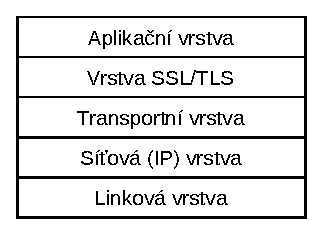
\includegraphics[width=0.3\textwidth]{fig/vrstvy-ssl}
  \caption{Vrstvy TCP/IP modelu s využitím SSL/TLS.}
 \label{fig:tls}
\end{figure}

Protokol TLS standardizuje IETF na základě původního protokolu SSL, který je
dnes již zastaralý~\cite{RFC7568}. Poslední verze protokolu TLS je
1.3~\cite{RFC8446}\footnote{Převyprávěná verze RFC 8446 je dostupná na \url{https://www.davidwong.fr/tls13/}}.

TLS vytváří obousměrný šifrovaný kanál mezi dvěma počítači, který zajišťuje:

\begin{itemize}

  \item Autentizaci: vždy se ověřuje identita serveru, identita klienta může být
  také ověřená. Pro ověřování se používají certifikáty X.509, které mohou být
  podepsány certifikační autoritou.

  \item Důvěrnost (utajení): po navázání spojení je obsah přenášené komunikace
  známý pouze komunikujícím stranám. Délka zpráv může být pozorovateli
  komunikace známá, TLS podporuje vycpávkový provoz.

  \item Integritu: Obsah zprávy není možné bez odhalení při přenosu upravit.

\end{itemize}

Samotný protokol TLS se skládá ze dvou podprotokolů:

\begin{itemize}

  \item \emph{Handshake protocol} se používá při navazování spojení a zajišťuje
  autentizaci komunikujících stran, domluvu kryptografických parametrů a
  sdílených klíčů.

  \item \emph{Record protocol} přenáší data mezi komunikujícími stranami.

\end{itemize}

\subsection{Certifikační autority}


Certifikační autorita (CA)\footnote{Text popisující CA je převzatý z~{\tt https://cs.wikipedia.org/wiki/Certifika\%C4\%8Dn\%C3\%AD\_autorita}.} je v asymetrické kryptografii subjekt, který vydává
digitální certifikáty (elektronicky podepsané veřejné šifrovací klíče), čímž
usnadňuje využívání Public Key Infrastructure (PKI) tak, že svojí autoritou
potvrzuje pravdivost údajů, které jsou ve volně dostupném veřejném klíči
uvedeny. Na základě principu přenosu důvěry tak můžeme důvěřovat
údajům uvedeným v digitálním certifikátu za předpokladu, že důvěřujeme samotné
certifikační autoritě.

Na Internetu působí mnoho komerčních certifikačních autorit, které obvykle mají
své veřejné klíče umístěny přímo ve webových prohlížečích a dalších programech,
čímž mohou uživateli zjednodušit rozhodování o míře důvěry webových serverů, ke
kterým se připojuje (ale též digitálně podepsaných e-mailů i jiných dat).
Existují též bezplatné certifikační autority nebo takové, které se řídí zákony
daného státu, vnitřními předpisy organizace a podobně.

Hodnota digitálního certifikátu je úměrná míře důvěry, kterou máme k údajům
v~něm uvedených. Proto je pro certifikační autoritu nejdůležitější důvěra, kterou
vůči svému okolí vzbuzuje (tj. že nevydá digitální certifikát s nepravdivými
údaji). Certifikační autorita proto musí adekvátním způsobem pečovat o svoji
důvěryhodnost, jinak by nebylo možné využít principu přenosu důvěry.

\subsection{Transparentnost certifikátů}

Aby bylo možné ověřit, že CA vydávají certifikáty poctivě, byl experimentálně
zaveden mechanismus transparentnosti certifikátů. Zapojené CA veřejně ohlašují
každý vystavený certifikát (případně precertifikát). Vydané certifikáty se
shromažďují v lozích (cerificate transparency log), kde je monitorovat nově
přidávané certifikáty a auditovat přítomnost certifikátu nalezených při
prohlížení webu.

%%%%%%%%%%%%%%%%%%%%%%%%%%%%%%%%%%%%%%
\section{Domain Name System}
\label{dns}
Cílem DNS je zajistit překlad mezi doménovým jménem a IP adresou. Dříve se jednalo především o~překlad hostname na IP adresu a naopak, tedy záznamy typu {\tt A}, {\tt AAAA}, {\tt PTR} \cite{rfc1035,rfc3596}. Dalším známým typem je {\tt MX}, který deleguje zodpovědnost za příjem e-mailové pošty dané domény. Tento typ se od předchozích tří odlišuje, protože se nejedná o~adresaci hosta, ale služby. Podobný význam mají i záznamy typu {\tt SRV}, které lze v~současnosti využít pro služby SIP a XMPP \cite{rfc2782}.

Mimo tyto typy záznamů existují i další. Některé jsou definovány již v~původním návrhu, jiné přidané později nebo význam původních typů vyžit pro další služby (např. {\tt TXT} využito pro distribuci veřejného klíče podepisování emailu DKIM \cite{rfc4871}).

\subsection{Klient}
Aby klient věděl, na který server se obrátit s~požadavkem na přeložení doménového jména na IP adresu či opačně, je součástí systému tzv. resolver. Tento resolver má několik konfiguračních souborů, z~nichž jmenujme {\tt /etc/hosts}, {\tt /etc/resolv.conf} a {\tt /etc/host.conf}.

První z~těchto souborů se používá pro statický překlad doménového jména na IP adresu. Formát souboru a další popis lze nalézt v~manuálových stránkách {\tt man hosts}.

Dynamický překlad, neboli překlad pomocí DNS serveru, vyžaduje existenci konfiguračního souboru {\tt /etc/resolv.conf}, který obvykle obsahuje jedenkrát volbu {\tt search} a jednu nebo více voleb {\tt nameserver}.
\begin{description}
  \item[search] definuje tzv. searchlist, neboli seznam domén (max. 6), které se budou prohledávat, pokud je požadavek na překlad neúplného doménového jména. Tedy má-li tato volba podobu {\tt search fit.vutbr.cz}, pak při pokusu přeložit jméno {\em merlin} se při neúspěchu pokusí systém také přeložit jméno {\em merlin.fit.vutbr.cz}.
  \item[nameserver] se uvádí právě s~jedním parametrem, který definuje IP adresu DNS serveru, který se systém pokusí kontaktovat. Může se jednat jak o~IPv4 tak o~IPv6 adresu.
\end{description}
Další možnosti, které může soubor obsahovat, lze nalézt v~manuálových stránkách {\tt man resolv.conf}.

V~souboru {\tt /etc/host.conf} lze definovat, v~jakém pořadí se předchozí dvě volby využijí. Standardně se nejprve zkouší statický překlad a poté dynamický. Toto výchozí nastavení umožňuje lokální předefinování překladu z doménového jména na IP adresu.

Pokud se síť na klientovi konfiguruje dynamicky, pak je soubor {\tt /etc/resolv.conf} upravován automaticky. Při statické konfiguraci musí být obsah souboru upraven ručně.

\subsection{Konfigurace serveru}
Konfigurace DNS se stává ze dvou částí -- konfigurace vlastností samotné aplikace a konfigurace obsluhovaných zón. Existuje mnoho různých variant implementací. V~laboratoři se bude pracovat s~implementací od ISC -- BIND.

Konfigurační soubor {\tt\bf named.conf} se na počítačích v~laboratořích nachází ve složce {\tt
/etc/bind/}. V Linuxové distribuci Kali tento soubor obsahuje vložené 3 soubory (pro konfiguraci voleb,
konfiguraci lokálních zón a konfiguraci výchozích zón).

%\begin{verbatim}
%
%acl "local" {
%  <prefix>/<délka prefixu>;
%};
%
%options {
%  listen-on-v6 { <ipv6 adresa lokálního rozhraní>; };
%  allow-query { local; };
%  allow-recursion { local; };
%  allow-transfer { none; };
%  allow-update { none; };
%  directory "/etc/namedb/working";
%  pid-file "/var/run/named/pid";
%}
%
%zone "." IN {
%  type hint;
%  file "/etc/namedb/named.root";
%};
%
%zone "localhost" IN {
%  type master;
%  file "/etc/namedb/master/localhost-forward.db";
%  notify no;
%};
%
%zone "127.in-addr.arpa" IN {
%  type master;
%  file "/etc/namedb/master/localhost-reverse.db";
%  notify no;
%};
%
%zone "0.ip6.arpa" IN {
%  type master;
%  file "/etc/namedb/master/localhost-reverse.db";
%  notify no;
%};
%
%zone "255.in-addr.arpa" IN {
%  type master;
%  file "/etc/namedb/master/empty.db";
%  notify no;
%};
%
%zone "0.in-addr.arpa" IN {
%  type master;
%  file "/etc/namedb/master/empty.db";
%  notify no;
%};
%
%\end{verbatim}

%Zóna typu {\tt hint} odkazuje na seznam tzv. root serverů, tedy takových serverů, které znají informace
%o všech registrovaných top-level doménách a dokáží říci, které servery jsou za tyto top-level domény
%zodpovědné. Zóna typu {\tt master} značí, že server je autoritativním serverem pro danou doménu.
%Mezi povinné záznamy pro takovou doménu patří záznam typu SOA a alespoň jeden NS odkazující na server samotný. Zároveň by měl být obsažen i záznam typu A pro tento server.
Další možnosti konfiguračního souboru naleznete v~manuálových stránkách {\tt man named.conf}.

\subsubsection{Zóna typu hint}
Asociuje se s~nejvyšší doménou v~rámci celé hierarchie. Pokud přijde na server požadavek, prohledá seznam spravovaných zón ostatních typů ({\em master}, {\em slave}, {\em forward}). Pokud záznam nenajde, vybere jeden z~kořenových serverů definovaný právě v~tomto typu zóny.

Soubor, který je vyžadován pro konfiguraci této domény lze získat například programem dig:
\begin{verbatim}
 dig +norec NS . @a.root-servers.net > /etc/bind/db.root
\end{verbatim}

\subsubsection{Lokálně obsluhovane zóny}
Tyto zóny lze rozdělit do dvou skupin -- {\bf loopback adresy} a {\bf ,,prázdné zóny''}. RFC 6303
\cite{rfc6303} je z~kategorie {\em best practice} a definuje, které zóny by měl být schopen DNS server
obsloužit sám a tím redukovat dotazy přeposílané na další servery. Ve většině případů jsou to zóny pro reverzní záznamy privátních IP adres.

%Výchozí soubor aplikace {\bf named} ve FreeBSD respektuje právě RFC 6303 a navíc doplňuje ještě další
%zóny. Například nealokované rozsahy IPv6 adres. Pro práci v~laboratoři nahraďte původní soubor {\tt
%/etc/namedb/named.conf} souborem {\tt /root/isa1/named.conf}, který je zkrácen a obsahuje pouze nezbytné definice.

\subsubsection{Vlastní zóna}
Aby server začal překládat vlastní zónu, je třeba přidat definici zóny do souboru {\tt named.conf.local} a vytvořit zónový soubor. Pokud se přidává zónový soubor pro doménu, je vhodné přidat i zónu pro reverzní záznamy.

\begin{verbatim}
zone "moje.domena.cz" {
  type master;
  file "/var/cache/bind/moje.domena.cz.zone";
};

zone "0.168.192.in-addr.arpa" {
  type master;
  file "/etc/bind/master/192.168.0.rev";
};
\end{verbatim}

Pro každou z~těchto zón se tvoří samostatný zónový soubor, jehož základní tvar má podobu:

%$ORIGIN <nazev domény>
\begin{verbatim}
$TTL 5m

@ IN  SOA <fqdn autoritativniho serveru>. <email správce>. (
  1   ; seriové číslo
  10h ; obnovovací interval pro sekundární servery
  10m ; prodleva, po které se sekundární server pokusí znova kontaktovat
      ; autoritativní server, pokud se předchozi spojení nezdařilo
  1w  ; jestliže se sekundárnímu serveru nepodaří kontaktovat autoritativní
      ; server během této doby, přestane vracet záznamy pro tuto doménu
  1h  ; původně výchozí TTL (nahrazeno $TTL), nově určuje
      ; NEGATIVNÍ TTL -- pro chybové odpovědi (např. NXDOMAIN)
  )

@ IN  NS <fqdn autoritativního serveru>
@ IN  NS <fqdn sekundárního serveru>

následuje seznam dalších záznamů
\end{verbatim}
Typ záznamu {\tt\bf SOA} definuje parametry zóny -- jméno autoritativního serveru a email správce domény. Všimněte si, že znak `{\tt @}' má zvláštní význam (zastupuje název domény). Z~tohoto důvodu se v~emailu správce nahrazuje znak `{\tt @}' za znak `{\tt .}' (tečka).

Záznam typu {\tt\bf NS} by měl být vždy obsažen alespoň jednou a to právě pro autoritativní server. Počet sekundárních serverů je libovolný. Tyto záznamy by také měly byt obsaženy v~nadřazené doméně, aby bylo možné nalézt server zodpovědný za danou poddoménu. Tedy kořenová doména obsahuje {\tt NS} záznamy pro domény nejvyšší úrovně {\em .cz, .com, .eu, \dots} a ty zase pro jednotlivé poddomény {\em google.com, seznam.cz, \dots}.

V~zónovém souboru se rozlišuje mezi relativním a absolutním jménem. O~jaký typ jména jde, se rozlišuje podle zakončení. Končí-li tečkou, je to jméno absolutní (plně kvalifikované). V~opačném případě jde o~jméno relativní a za to se vždy doplní obsah definován v~{\tt \$ORIGIN}. Jestliže není definován, použije se název, který je definován u~názvu zóny v~souboru {\tt named.conf}.

Další záznamy mají obecný tvar:
\begin{verbatim}
jméno  ttl  třída  typ  <na typu závislá data>
\end{verbatim}
Jméno běžně bývá ve tvaru relativním. Pokud není hodnota TTL jiná než je výchozí pro celou zónu, pak se může vynechat. Třída záznamu se běžně používá pouze {\tt IN} (Internet). Kromě typu SOA a NS, se v~laboratorním cvičení použijí záznamy typu {\tt A}, {\tt PTR} a volitelně {\tt AAAA}. Typ {\tt AAAA} se chová stejně jako záznam typu {\tt A}, který se používá pro IPv4. Typově závislými daty je v~tomto případě adresa IPv6, resp. IPv4. Příklad:
\begin{verbatim}
host  IN A  192.168.0.1
\end{verbatim}
\begin{verbatim}
host  IN AAAA  fd12:1234::1
\end{verbatim}
Typ {\tt PTR} nerozlišuje, zda se jedná o~IPv6 nebo IPv4 adresu. Pro tento případ se typově závislá data chovají stejně jako jméno na začátku záznamu. V~tomto případě se ale vždy zapisuje v~plném tvaru. Další zvláštností PTR záznamu, který je vidět i v~názvu zóny, je, že se hodnoty zapisují v~obráceném pořadí a každá hodnota je oddělená tečkou. Obrácené pořadí je kvůli vyhodnocování záznamů od konce a tečka mezi každým číslem dovoluje snadnější delegaci podsítě na jiný DNS server. Příklad:
\begin{verbatim}
1		IN	PTR	host.moje.domena.cz.
\end{verbatim}

Pro IPv6 můžete využít:
\begin{verbatim}
$ORIGIN 0.0.0.0.0.0.0.0.4.3.2.1.2.1.d.f.ip6.arpa.
1.0.0.0.0.0.0.0.0.0.0.0.0.0.0.0   IN PTR host.moje.domena.cz.
\end{verbatim}
Oproti tomu záznamy
\begin{verbatim}
$ORIGIN 0.0.0.0.0.0.0.0.4.3.2.1.2.1.d.f.ip6.arpa.
2.0.0.0.0.0.0.0.0.0.0.0.0.0.0.0   IN PTR host
1.0.0.0.0.0.0.0.0.0.0.0.0.0.0.0   IN PTR host.moje.domena.cz
\end{verbatim}
jsou neplatné, protože na dotaz by vrátily:
{\small
\begin{verbatim}
1.0.0.0.0.0.0.0.0.0.0.0.0.0.0.0.0.0.0.0.0.0.0.0.4.3.2.1.2.1.d.f.ip6.arpa. IN PTR
                                              host.0.0.0.0.0.0.0.0.4.3.2.1.2.1.d.f.ip6.arpa.
1.0.0.0.0.0.0.0.0.0.0.0.0.0.0.0.0.0.0.0.0.0.0.0.4.3.2.1.2.1.d.f.ip6.arpa. IN PTR
                               host.moje.domena.cz.0.0.0.0.0.0.0.0.4.3.2.1.2.1.d.f.ip6.arpa.
\end{verbatim}}

Příklad PTR záznamu pro IPv4 je:
\begin{verbatim}
19.176.229.147.in-addr.arpa. IN	PTR	merlin.fit.vutbr.cz.
\end{verbatim}

Po každé změně zónového souboru by se vždy mělo upravit i sériové číslo zóny a to tak, aby bylo vždy větší než předchozí hodnota. Také je nutné aplikaci načíst změněnou konfiguraci.
\begin{verbatim}
systemctl restart bind9.service
\end{verbatim}


\section{DNS Security Extensions (DNSSec)}
\label{dnssec}

DNS je službou, která si z~inulosti nese různé problémy. Jedním z~nich je
nezabezpečení této služby vůči útokům s~podvržením záznamu.
DNSSEC rozšiřuje službu DNS o~bezpečnostní prvky, jejichž cílem je zabránit
útokům využívající podvržené záznamy v DNS. Obrana spočívá v~zavedení
asymetrické kryptografie pro podepisování zón. Přesněji řečeno se podepíše každý
záznam v~zóně a tyto podpisy se zveřejní jako speciální typ záznamu. Protože není možné, aby resolver měl uložený veřejný klíč od každé zóny, používá se metoda sestavení důvěryhodného řetězce s~tím, že resolver v~tomto případě potřebuje mít uložen pouze veřejný klíč nejvyšší domény. Aby tento systém fungoval, musí nadřazená doména obsahovat nejen záznamy typu {\tt NS} ale i záznam typu {\tt DS} -- speciální typ záznamu obsahující hash klíče a název domény. Principiálně samozřejmě může mít resolver uložen veřejné klíče více zón.

Pro vytvoření klíčů a podepsaní zóny není třeba zpracovávat každý záznam samostatně. Součástí balíčku {\em bind} jsou aplikace, kterým stačí zadat vhodné parametry, a ty zajistí vytvoření všech potřebných souborů. Pak již jen stačí správně nakonfigurovat aplikaci {\tt named}, aby tyto soubory používala.

\subsection{Klíče}
Není to nezbytně nutné, ale obecně se doporučuje používat v~DNSSec dva typy klíčů:
\begin{itemize}
  \item Key Signing Key (KSK) a
  \item Zone Signing Key (ZSK).
\end{itemize}
Ve své podstatě se tyto klíče liší jen v~jediném bitu (SEP -- Secure Entry
Point), který říká, že od tohoto místa může byt zahájeno sestavovaní
důvěryhodného řetězce. V~praxi se tyto dva klíče liší ještě další vlastností,
která se určuje při jejích vytváření -- délkou. Důvodem je vztah mezi délkou
klíče, bezpečností a výpočetními nároky. Delší klíč je sice bezpečnější, ale
zároveň má vyšší nároky na výkon a naopak. Protože k~překladu DNS dochází velice
často, není žádoucí, aby tato operace byla náročná na výpočetní zdroje. Proto
byl zvolen postup, kdy klíč, který je často používán, je sice slabší, ale na
druhou stranu jej lze měnit relativně často bez větších obtíží, a je-li čas
nutný k~jeho prolomení hrubou sílou delší, než délka jeho platnosti, pak jeho prolomení nepředstavuje problém -- tímto klíčem je klíč pro podepisování zóny (ZSK). Druhý klíč (KSK) se použije pouze pro podepsání ZSK, což znamená, že se nepoužívá tak často. V~důsledku tento klíč může být delší a proto i odolnější vůči prolomení. Výměna tohoto klíče je obvykle trošku složitější, neboť vyžaduje spolupráci se správcem nadřazené domény. Čas, po kterém je nutné klíče obměnit, není explicitně definován a stejně tak klíče neobsahují časové vymezení platnosti. Po jaké době provést výměnu klíčů je tedy v~režii správce domény a víceméně to závisí i na frekvenci používaní klíče k~podpisu. Dochází-li v~doméně k~častým změnám a tedy i k~častému podepisování, je vhodné měnit klíče častěji.

Pro vygenerování klíčů je v~balíku {\em bind} k~dispozici aplikace {\tt dnssec-keygen}, které stačí jediný parametr\footnote{Závisí na implementaci, v~některých systémech může požadovat více parametrů.} -- název domény. Další užitečné parametry jsou:
\begin{description}
  \item[{\tt -f KSK}] pokud má mít vygenerovaný klíč nastaven SEP bit,
  \item[{\tt -b <číslo>}] pro nastavení délky klíče,
  \item[{\tt -a <algoritmus>}] pro výběr algoritmu a 
  \item[{\tt -r}] kterým se nastaví zdroj náhodných dat (standardně se použije {\tt /dev/random}, který je blokující, pokud nemá dostatek entropie a může být vhodné nahradit ho {\tt /dev/urandom}).
\end{description}
Pro získaní seznamu dalších možností stačí spustit bez parametru. Po spuštění aplikace se správnými parametry je vypsán na výstup řetězec, který se skládá z~názvu domény, číselného kódu použitého algoritmu a identifikačního čísla klíče. Kromě toho vytvoří dva soubory, jejíchž jména začínají vypsaným řetězcem a končí příponami {\tt .key} a {\tt .private}. První z~nich obsahuje veřejný klíč a ten druhý privátní. Podle toho by se také s~těmito klíči mělo zacházet (omezit přístup k~privátnímu klíči, apod.). Příkazy:

\begin{verbatim}
dnssec-keygen -r /dev/urandom -a RSASHA1 -b 2048 -f KSK example.com
dnssec-keygen -r /dev/urandom -a RSASHA1 -b 1024 example.com
\end{verbatim}
vytvoří čtyři soubory, kde první pár je KSK a druhý ZSK. Oba klíče je třeba
zveřejnit v~zóně. Vypsáním obsahu souborů s~příponou {\tt .key} zjistíte, že
záznamy již mají tvar požadovaný pro zápis do zóny. Obsah těchto souboru se může
buďto zkopírovat do zónového souboru a nebo je připojit pomocí direktivy {\tt
\$INCLUDE}, např:

\begin{verbatim}
cat Kexample.com.+005+06487.key >> /var/cache/bind/example.com
cat Kexample.com.+005+32883.key >> /var/cache/bind/example.com
\end{verbatim}

Alternativně přidejte do souboru {\tt /var/cache/bind/example.com} řádek:

\begin{verbatim}
$INCLUDE Kexample.com.+005+06487.key;
$INCLUDE Kexample.com.+005+32883.key;
\end{verbatim}

Nyní už jen stačí zónový soubor podepsat. To se provede příkazem {\tt
dnssec-signzone}, kterému se pouze předá parametrem název souboru, který obsahuje podepisovanou zónu. Pokud se název souboru neshoduje s~názvem zóny, pak je třeba použít ještě parametr {\tt -o}, kterým se určí název podepisované zóny. Pro podpis zóny se použijí automaticky ty klíče, jejichž veřejné části byly vloženy do zónového souboru (viz odstavec výše).
\begin{verbatim}
dnssec-signzone -o example.com labXX.zone
\end{verbatim}
Parametr \verb|-o| specifikuje origin a \verb|labXX.zone| je jméno zónového
souboru (vstupního souboru).
Výstupem tohoto příkazu je soubor se stejným názvem jako vstupní soubor rozšířený o~příponu {\em .signed}. Pokud je požadován jiný název výstupního souboru, lze toho docílit volbou {\tt -f}. Takto vzniklý soubor má požadovaný tvar zónového souboru. Stačí jen upravit {\tt /etc/namedb/named.conf}, aby místo původního zónového souboru (bez podpisů) začal používat nově vzniklý soubor, který obsahuje i podpisy záznamů.

V~souboru podepsané zóny se objevily nové typy záznamů {\tt DNSKEY}, {\tt RRSIG} a {\tt NSEC}. První z~nich je typ, který nese data o~veřejné části klíče. {\tt RRSIG} obsahuje samotný podpis plus další informace -- typ podepsaného záznamu, jeho TTL, časy od kdy a do kdy je podpis platný a ID klíče, kterým byl podpis proveden. Poslední ze záznamu ({\tt NSEC}) obsahuje informaci o~následujícím záznamu v~abecedně seřazené zóně. Tento záznam se využívá při odpovědi pro dotaz na neexistující záznam. Protože součásti podpisu je i časové vymezeni jeho platnosti, je nutné provádět znovupodepsání zóny. To by se mělo provést dříve, než vyprší platnost starých záznamů (nutné počítat se zkrácením hodnotou TTL, po kterou mohou být staré záznamy uloženy v~cache paměti).

V~tuto chvílí je již zóna podepsána a je možné ji začít používat. Ovšem resolver, který bude ověřovat, že je zóna dobře podepsaná, nemá k~dispozici veřejný klíč (z~jiného bezpečného zdroje), a nadřazená zóna neobsahuje informaci o~použitém klíči a není proto možné sestavit důvěryhodný řetězec. Zbývá požádat správce nadřazené zóny o~zveřejnění {\tt DS} záznamu. Tento DS záznam se vytváří pro KSK klíč. Při podpisu zóny vznikne také soubor začínající řetězcem {\em dsset-} a končící názvem zóny. Tento soubor obsahuje {\tt DS} záznamy, které je potřeba zveřejnit. Tyto záznamy lze také získat příkazem {\tt dnssec-dsfromkey}. Pokud se nepoužijí žádné volby, pak tento program standardně vypíše na výstup dva DS záznamy ve stejné formě, jako je ve výše uvedeném souboru (jeden s~použitím algoritmu SHA-1 a druhý s~SHA-256). První z~nich by měl být zveřejněn povinně.
\begin{verbatim}
dnssec-dsfromkey <název souboru s KSK klíčem>
\end{verbatim}
Předání DS záznamů ke správci nadřazené domény se běžně provádí "out-of-band". Samotné záznamy jsou tedy přidávány ručně. Tento proces je nutné provádět i v~případech výměny klíčů, což může vést k~chybám při přidání nového klíče. Proces lze však automatizovat 
pomocí {\tt CDS} a {\tt CDNSKEY} záznamů \cite{rfc7344}, \cite{rfc8078}. Tyto záznamy obsahují stejná data jako příslušné {\tt DS}/{\tt DNSKEY} záznamy, avšak je možné tato data předat standardní důvěryhodnou cestou. Servery nadřazené domény tyto záznamy využijí k~synchronizaci uložených DS/DNSKEY dat. Poté je možné CDS a CDNSKEY záznamy odebrat.

\subsubsection*{Výměna klíčů}
Jak bylo uvedeno výše, používají se obvykle dva typy klíčů, kdy jeden je slabší a druhy silnější. Oba tyto klíče je třeba obměňovat, aby nedošlo ke kompromitování zóny. Slabší z~klíčů, ZSK, je třeba měnit častěji, ale vzhledem k~tomu, že se změnou tohoto klíče není svázaná nutnost změny v~nadřazené zóně, je tento krok relativně jednodušší (alespoň po administrativní stránce).

Při vyměně klíčů je nutné zajistit, aby klienti měli vždy k~dispozici klíč, kterým jsou data podepsána. Způsoby, jak toho dosáhnout jdou dva -- buďto podepsat data starým i novým klíčem, nebo nejprve zveřejnit nový klíč, počkat až se klíč rozšíří, a pak jej začít používat k~podepisování zóny. Varianta, kdy se data podepíší starým i novým klíčem, je sice rychlejší, ale rovněž znamená, že zónový soubor zvětší svou velikost (a to téměř dvojnásobně). Z~tohoto důvodu se tento způsob používá pouze pro výměnu KSK klíčů. Druhý způsob vyžaduje více časů, ale předchází zvětšování zónového souboru -- běžně se používá pro výměnu ZSK.

\subsection{Ověřování podepsané zóny}
Bind od verze 9.5 má validaci zapnutou implicitně. Liší se ovšem způsob zpracování veřejného klíče. V~současné době již je podepsána zóna {\tt root}, a není proto nezbytně nutné zabývat se distribucí klíčů pomocí DLV registrů.

Do verze 9.6 se používala direktiva {\em trusted-keys} v~konfiguračním souboru, která měla obdobný formát jako {\tt DNSSEC} záznam. Při použití této možnosti je nutné hlídat, zda nedošlo ke změně klíče root zóny a v~tomto případě tento klíč obnovit. Od verze 9.7 se používá volba {\em managed-keys}, která má stejný formát, a funguje v~podstatě stejně jako {\em trusted-keys}, ale navíc dovoluje použití automatického sledování změny klíče root zóny definované v~RFC 5011 a nevyžaduje zásah operátora v~případě obměny \cite{RFC5011}.

%\subsubsection*{Poznámka}
%Pro práci v~laboratoří bude server {\em isa} nastaven jako nejvyšší důvěryhodný server (jeho klíč bude nainstalován na pracovních stanicích) a bude mít k~dispozici DS záznamy pro KSK před připravené na stanicích. Bude-li použit tento klíč pro podpis zóny, bude validující resolver schopen sestavit důvěryhodný řetězec a ověřit DNS záznamy.
%

%
% ISA - program laboratorn�ho cvi�en� �.3
%
% (c) Petr Matousek, 2008
%

\documentclass{article}[10]
\usepackage{a4wide}
\usepackage{czech}
\usepackage{epsfig}

%\include{macro_lecture}
\title{ISA - Laboratorn� cvi�en� �.3\\
{\bf\large Spr�va s�t�}}

\author{p�ipravili Mat�j Gr�gr, Martin ��dn�k a Libor Pol��k\footnote{FIT VUT v Brn�,
    {\tt\{igregr,izadnik,ipolcak\}@fit.vutbr.cz}}}
    \date{Zimn� semestr 2010/2011, verze 1.2}
\begin{document}
\maketitle

\section*{C�l laboratorn�ho cvi�en�}
\begin{itemize}
  \item sezn�mit se s n�stroji pro spr�vu s�t�
  \item nau�it se pracovat s programem syslog
  \item konfigurace n�stroj� pro pr�ci s protokolem SNMP
  \item otestovat pr�ci se syslog a SNMP
  \item sezn�mit se s protokolem NetFlow
  \item nau�it se pracovat s n�stroji {\tt nfsen} a {\tt nfdump}
\end{itemize}

\section*{Pokyny}
\begin{itemize}
  \item Do zad�n� nepi�te, slou�� pro dal�� skupiny. PDF verzi zad�n�
  i �ablony konfigura�n�ch soubor� lze naj�t v IS u p�edm�tu ISA.
  \item Na konci laboratorn�ho cvi�en� nezapome�te na posledn� bod,
  tj. na {\bf Ukon�en� pr�ce v laborato�i}!
\end{itemize}

\newpage
%\section{Laboratorn� �lohy}
\section{Syslog}
  \begin{itemize}
  	\item �kol: 
    \begin{itemize}
      \item Sezn�mit se s  protokolem Syslog, kter� slou�� pro p�enos
      logovac�ch zpr�v ze spravovan�ch za��zen�. Pojmem Syslog je �asto ozna�ov�no tak�
      programov� vybaven� implementuj�c� samotn� p�enos, t��d�n� a ukl�d�n� zpr�v na disk.
      \item Rozd�lte se do dvojic. V ka�d� dvojici zvolte jednu stanici jako klient a
      druhou jako server a nakonfigurujte p�epos�l�n� ve�ker�ch Syslog zpr�v 
      z klienta na server. M�jte na pam�ti mo�n� zneu�it� Syslog protokolu �to�n�kem a omezte
      na stran� serveru p��jem pouze na zpr�vy od dan�ho klienta
      a klientovi zamezte p��jem jak�chkoliv zpr�v ze s�t�.
      \item Pro pr�ci vyu�ijte n�stroj {\tt syslogd}, kter� bude slou�it jako server i klient. K
      otestov�n� vyu�ijte n�stroj {\tt logger}.
      \item Na klientovi n�sledn� omezte p�epos�l�n� pouze na zpr�vy konkr�tn�ho typu.
    \end{itemize}
  	\item P��kazy:
	   \begin{itemize}
    		\item {\tt syslogd(8)} -- Syslog d�mon.
    		\item {\tt syslog.conf(5)} -- Popis konfigurace Syslog d�mona.
    		\item {\tt logger(1)} -- N�stroj pro generov�n� Syslog zpr�v.
    		\item {\tt tcpdump(1)}
  		\end{itemize}
  	\item Postup:
	   \begin{enumerate}
    		\item Rozd�lte se do dvojic a ur�ete server a klient stanici.
    		\item Povolte spu�t�n� Syslogd d�mona na serveru i klientovi, tj. p�idejte
         n�sleduj�c� ��dek do {\tt /etc/rc.conf}:
\begin{verbatim}
  syslogd_enable="YES"
\end{verbatim} 
    		\item {\bf Na serveru} omezte p��jem Syslog zpr�v pouze od konkr�tn�ho klienta, tj. p�idejte do {\tt /etc/rc.conf}:
\begin{verbatim}
  syslogd_flags="-a <plne_domenove_jmeno_klienta> -vv"
\end{verbatim} 


    		\item {\bf Na serveru} nakonfigurujte syslog d�mona tak, aby ukl�dal ve�ker� zpr�vy
         od klienta do souboru {\tt /var/log/logclient.log}. P�i editaci souboru {\tt
         /etc/syslog.conf} pou�ijte jako odd�lova� v�hradn�
         tabul�tor nikoliv mezeru. Na za��tek souboru {\tt /etc/syslog.conf} p�idejte n�sleduj�c� pravidlo a odd�lte ho od zbytku pravidel
         pr�zdn�m ��dkem:
\begin{verbatim}
 +<plne_domenove_jmeno_klienta>
 *.*<TAB><TAB><TAB>/var/log/logclient.log
\end{verbatim} 

    		\item {\bf Na serveru} je nutn� vytvo�it soubor pro logov�n�, v opa�n�m p��pad� by
         Syslog d�mon do souboru nezapisoval:
\begin{verbatim}
 touch /var/log/logclient.log
\end{verbatim} 

    		\item {\bf Na klientovi} zaka�te programu syslogd naslouchat na s��ov�m soketu, tj. p�idejte do {\tt /etc/rc.conf}:
\begin{verbatim}
 syslogd_flags="-s -vv"
\end{verbatim} 

    		\item {\bf Na klientovi} nakonfigurujte Syslog d�mona tak, aby odes�lal ve�ker� zpr�vy
         z klienta na server. Jako odd�lova� pou�ijte v�hradn�
         tabul�tor nikoliv mezery. Do souboru {\tt /etc/syslog.conf} p�idejte n�sleduj�c� pravidlo:
\begin{verbatim} 
 *.*<TAB><TAB><TAB>@<plne_domenove_jmeno_serveru>
\end{verbatim}

\newpage
    		\item {\bf Na serveru i klientovi} restartujte Syslog d�mona: 
\begin{verbatim} 
 /etc/rc.d/syslogd restart
\end{verbatim} 

    		\item {\bf Z klienta} ov��te spr�vnou konfiguraci vygenerov�n�m testovac� Syslog 
         zpr�vy pomoc� n�stroje {\tt logger}:
\begin{verbatim} 
 logger "Toto je testovaci zprava z klienta"
\end{verbatim} 
        
    		\item Zpr�va byla p�eposl�na na server, kde ji lze naj�t na konci souboru
         {\tt /var/log/logclient.log}.

\begin{verbatim} 
 tail -f /var/log/logclient.log
\end{verbatim} 

    		\item  Na klientovi pokra�ujte v generov�n� Syslog zpr�v a 
         na serveru sledujte p��choz� Syslog zpr�vy pomoc� {\tt tcpdump}. Na jak�m
         portu a jak�m protokolem jsou Syslog zpr�vy zas�l�ny. D�le vysv�tlete,
         co znamen� zv��en� v�skyt DNS komunikace po ka�d�m p��chodu Syslog
         paketu~\footnote{Jedn� se o p�eklad zdrojov� IP adresy Syslog paketu na dom�nov�
         jm�no, aby bylo mo�n� ov��it shodu jmen povolen�ch klient�}.

    		\item Otev�ete si manu�lovou str�nku syslog.conf a zjist�te, jak� za��zen� a priority
         zpr�v Syslog poskytuje. 
\begin{verbatim} 
 man syslog.conf
\end{verbatim} 
        
         \item Ze znalosti za��zen� a priorit nakonfigurujte klienta, aby pos�lal na server 
         pouze zpr�vy
         p�i selh�n� autentizace, tj. upravte ji� existuj�c� pravidlo pro p�epos�l�n�
         ve�ker�ch zpr�v na server v souboru {\tt /etc/syslog.conf}. Nezapome�te restartovat Syslog d�mona. 
         
\begin{verbatim} 
 Syntax pravidel: <facility>.<priority><TAB><TAB><TAB><action>
\end{verbatim} 
         \item Ze serveru se
         n�sledn� pokuste o ne�sp�n� ssh p�ipojen� na klienta a pod�vejte se do souboru {\tt /var/log/logclient.log} jakou zpr�vu
          zaslal klient serveru.


	   \end{enumerate}
   \end{itemize}

\newpage

\section{SNMP}
  \begin{itemize}
  	\item �kol: 
    \begin{itemize}
      \item Sezn�mit se s  protokolem SNMP, kter� slou�� pro p�enos
      informac� o stavu spravovan�ch za��zen� (nap�. hodnot ��ta��). B�hem tohoto cvi�en� si
      vyzkou��te pr�ci se synchronn�mi SNMP ud�lostmi, tj. model komunikace dotaz-odpov��.
      \item Ka�dou stanici nakonfigurujte tak, aby lok�ln� umo��ovala �ten� i z�pis SNMP
      prom�nn�ch a p�i vzd�len�m p��stupu k SNMP prom�nn�m pouze �ten�.
    \end{itemize}
  	\item P��kazy:
	   \begin{itemize}
    		\item {\tt snmpd(8)} -- SNMP d�mon.
    		\item {\tt snmpd.conf(5)} -- Popis konfigurace SNMP d�mona.
    		\item {\tt snmpwalk(1)} -- N�stroj pro proch�zen� a z�sk�v�n� podstromu hodnot SNMP
         prom�nn�ch.
    		\item {\tt snmpget(1)} -- N�stroj pro z�sk�n� hodnoty SNMP prom�nn�.
    		\item {\tt snmpset(1)} -- N�stroj pro zm�nu hodnoty SNMP prom�nn�.
  		\end{itemize}
  	\item Postup:
	   \begin{enumerate}
         \item Povolte spu�t�n� SNMP d�mona, tj. p�idejte n�sleduj�c� ��dek do {\tt /etc/rc.conf}:
\begin{verbatim}
  snmpd_enable="YES"
\end{verbatim} 
         \item Zkop�rujte soubor {\tt /usr/local/share/snmp/snmpd.conf.example} obsahuj�c� p��klad
         konfigurace SNMP d�mona do {\tt /usr/local/etc/snmp/snmpd.conf}.
   		
    		\item Otev�ete si soubor {\tt /usr/local/etc/snmp/snmpd.conf} pro editaci a postupn�
         v n�m prove�te z�kladn� konfiguraci:
  		   \begin{enumerate}
    		   \item Zvolte si vlastn� n�zev komunity - nap�. PUBLIC
           \item Nastavte agenta, aby poslouchal na v�ech lok�ln�ch adres�ch \texttt{agentAddress
           udp:0.0.0.0:161}
    		   \item Namapujte s�t�, ze kter�ch bude mo�n� p�istupovat k SNMP
           hodnot�m. Povolte po��ta��m v u�ebn� z�pis pro �ten� {\tt rocommunity
           <CUMMUNITY> 10.10.10.0/24} a lok�ln�mu po��ta�i i z�pis {\tt rwcommunity <CUMMUNITY>
           localhost}
           \item V konfigura�n�m souboru je�t� nastavte SNMP prom�nn�
           \texttt{syslocation} a \texttt{syscontact} na V�mi vymy�len� hodnoty.
  		   \end{enumerate}
    		\item Spus�te d�mona {\tt snmpd}.
\begin{verbatim}
  /usr/local/etc/rc.d/snmpd start
\end{verbatim} 
    		\item Ov��te, �e d�mon b��. Na kter�ch portech naslouch�?
\begin{verbatim}
  /usr/local/etc/rc.d/snmpd status
  sockstat | grep snmpd
  ps -ax | grep snmpd
\end{verbatim} 
          \item P��kazem {\tt snmpwalk} p�e�t�te podstrom {\tt system} a zjist�te jak v�
          soused nastavil prom�nn� {\tt sysLocation} a {\tt sysContact}. Nap�.:
\begin{verbatim}
  snmpwalk -v 1 -c PUBLIC h01 system
  snmpwalk -v 1 -c <nazev_komunity> <domenove_jmeno> system
  snmpwalk -v 1 -c <nazev_komunity> <domenove_jmeno> system.sysLocation
  snmpwalk -v 1 -c <nazev_komunity> <domenove_jmeno> system.sysContact
\end{verbatim}

\newpage
          \item Pokud zn�te OID (Object Identifier) prom�nn� v datab�zi MIB (Management Information Base), pak
          m��ete z�skat hodnotu t�to prom�nn�
          p��mo pomoc� {\tt snmpget}, nap�. po�et byt� p�ijat�ch na rozhran� em0:
\begin{verbatim}
  snmpwalk -v 1 -c <nazev_komunity> \
           <domenove_jmeno_souseda> .1.3.6.1.2.1.2.2.1.16
  snmpget -v 1 -c <nazev_komunity> \
           <domenove_jmeno_souseda> .1.3.6.1.2.1.2.2.1.16.1
\end{verbatim}
          \item Zjist�te dal�� informace, nap��klad nastavenou MAC adresu (ifPhysAddress) na po��ta�i Va�eho
          souseda. Pro z�sk�n� pot�ebn�ho OID vyu�ijte webov� rozhran� Network management MIB
          nach�zej�c� se zde:
\begin{verbatim}
          http://www.oidview.com/mibs/0/RFC1213-MIB.html
\end{verbatim}
          \item Zkuste nastavit sv�mu sousedovi prom�nnou popisuj�c� n�zev jeho po��ta�e
          pomoc� n�stroje {\tt snmpset}:
\begin{verbatim}
  snmpget -v 1 -c <nazev_komunity> <domenove_jmeno_souseda> system.sysName.0
  snmpset -v 1 -c <nazev_komunity> <domenove_jmeno_souseda> \
          system.sysName.0 s <nove_jmeno>
\end{verbatim}
          \item Pro� p�edchoz� pokus o nastaven� prom�nn� sousedovi selhal? Zkuste nyn�
          nastavit svoji prom�nnou popisuj�c� n�zev Va�eho po��ta�e
          pomoc� n�stroje {\tt snmpset}:
\begin{verbatim}
  snmpget -v 1 -c <nazev_komunity> localhost system.sysName.0
  snmpset -v 1 -c <nazev_komunity> \
          localhost system.sysName.0 s <nove_jmeno_pocitace>
  snmpget -v 1 -c <nazev_komunity> localhost system.sysName.0
\end{verbatim}

\end{enumerate}
\end{itemize}
\newpage

\section{NetFlow}
  \begin{itemize}
  	\item �kol:
    	\begin{itemize}
      		\item Sezn�mit se mo�nostmi m��en� provozu pomoc� NetFlow. NetFlow slou�� pro
            p�enos statistik o jednotliv�ch toc�ch dat vznikaj�c�ch p�i komunikaci po s�ti.
            Z�znamy NetFlow, s nimi� budete b�hem cvi�en� pracovat, jsou
            po��zeny z napojen� s�t� VUT a anonymizov�ny. V druh� ��sti �kolu
            budete pracovat s daty po��zen�mi sondou FlowMon, kter� monitoruje
            d�n� v s�ti spole�nost� INVEA-TECH.
      		\item Sezn�mit se s n�strojem {\tt nfsen}, kter� graficky zobrazuje z�znamy
            NetFlow ve webov�m prohl��e�i. Sezn�mit se s n�strojem {\tt nfdump}, kter� slou�� k dotazov�n� na ulo�en� data NetFlow.
    	\end{itemize}
  	\item P��kazy:
  		\begin{itemize}
    		\item {\tt nfdump}
  		\end{itemize}
  	\item Postup:
  		\begin{enumerate}
			\item Nau�te se pou��vat n�stroj {\tt nfdump}, kter� slou�� k dotazovan� se nad z�znamy NetFlow.
				\begin{enumerate}
					\item Na Va�em po��ta�i se v adres��i {\tt /home/user/isa3/netflow} nach�z�
               \footnote{Nen�-li tomu tak, adres�� vytvo�te. Netflow data
               z�skejte pomoc� p��kaz� {\tt fetch
               http://FIXME} a {\tt tar xvf
               nfcapd-isa.tar}}
               anonymizovan� kolekce NetFlow dat. Tento adres�� bude vstupem programu {\tt
               nfdump}, kter� vyu�jte ke kladen� dotaz� nad NetFlow daty.
					\item Prostudujte manu�lovou str�nku n�stroje {\tt nfdump}.
					\item Dota�te se na n�sleduj�c� statistiky. TOP 20 IP adres podle po�tu p�enesen�ch bajt�. 
						\begin{itemize}
							\item V manu�lov� str�nce si najd�te, co d�laj� p�ep�na�e {\tt -R , -s, -n}.
							\item Nezapome�te, �e zpracov�v�te n�kolik soubor� o celkov�
              velikosti 600\,MB, tedy vytvo�en� statistiky chv�li potrv�!
						\end{itemize}
					\item Zjist�te, jak velk� datov� p�enosy p�ipadaj� na jednotliv� protokoly. (Statistika protokol�)
						\begin{itemize}
							\item V�imn�te si rozd�l� v pod�lech podle tok� a podle p�enesen�ch bajt�.
						\end{itemize}
					\item Na z�klad� z�skan�ch statistik se zamyslete nad velikost� s�t�.
               \footnote{Jedn� se o anonymizovan� data z p�te�n� s�t� VUT
               z�skan� za 1 hodinu provozu od 21 hodin} 
					\item Zam��te se na konkr�tn� stanici v s�ti, nap�. {\tt 194.179.74.239} a
               zjist�te, s k�m komunikovala, a odhalte podez�elou aktivitu tohoto u�ivatele.
               \footnote{P��li� mnoho jedno paketov�ch telnet spojen� b�hem kr�tk� doby na r�zn� po��ta�e ale stejn� port 23 ukazuje na skenovac� aktivitu �to�n�ka.}
\begin{verbatim}
 nfdump -R /home/user/isa3/netflow -o long -c 100 \
 "src ip 194.179.74.239"
\end{verbatim} 

				\end{enumerate}
  		\item P�ihla�te se na sondu FlowMon, b��c� ve spole�nosti INVEA TECH
  			\begin{enumerate}
  	   			\item webov� str�nka: {\tt
              https://www.flowmon.com/en/try-online-demo/}, FIXME kliknout na
                {\bf FlowMon Monitoring Center}, login: {\tt FIXME}, heslo: {\tt
                FIXME}. Nem��te ��dn� nastaven�.
  	   			\item Seznamte se s jednotliv�mi str�nkami, kter� vytv��� program {\tt
                nfsen}.
                Zam��te se na:
                   \begin{itemize}
                     \item {\bf Graphs} -- poskytuje dlouhodob� pohled na trendy v s��ov�m provozu
                     \item {\bf Details} -- nab�z� detailn� pohled na aktu�ln� provoz s mo�nost�
                     rozd�len� provozu na podle TCP, UDP, ICMP, d�le pak mo�nost dotazovat
                     se na TOP N statistiky nebo filtrovat a agregovat z�znamy.
                     \item {\bf Profile} -- Toto menu umo��uje filtrovat a ozna�it
                     barvou specifick� druhy provozu identifikovan� pomoc� ��sla portu a
                     protokolu.
                     \item {\bf Stats} -- tato str�nka zobrazuje nastaven� profilu a
                     umo��uje ho m�nit
                   \end{itemize}
             \item �koly:
                \begin{itemize}
                   \item Zjist�te, jak� IM protokoly se v t�to s�ti pou��vaj�.
                   \item Zjist�te, jak� P2P protokoly se v t�to s�ti pou��vaj�.
                   \item Kter� protokol transportn� vrstvy se pou��v�
                   nej�ast�ji? Jak� m� p�ibli�n� pod�l na celkov�m provozu v
                   s�ti? Jak se tento pod�l m�n� v pr�b�hu dne, t�dne? Zamyslete
                   se, pro� tomu tak je.
                \end{itemize}
  			\end{enumerate}       
		\end{enumerate}	
	\item Pro z�jemce:
		\begin{itemize}
			\item Z�jemci si mohou na str�nce {\tt https://demo.invea.cz} proj�t
      ostatn� moduly vystav�n� nad protokolem. Nem��te ��dn� nastaven�.
		\end{itemize}
	\end{itemize}
 
\section*{Ukon�en� pr�ce v laborato�i}
\begin{itemize}
  \item Pod u�ivatelem {\tt root} spus�te d�vku {\tt /root/isa3/isa3} pro zru�en�
  vytvo�en�ch konfigura�n�ch soubor� a pro vypnut� po��ta�e.
\end{itemize}

\end{document}


%%%%%%%%%%%%%%%%%%%%%%%%%%%%%%%%%%%%%%
\section{Signalizační protokol SIP}
\label{sip}
Session Initiation Protocol (SIP, RFC 3261, červen 2002) je textový aplikační protokol pro signalizaci VoIP, který provádí:
\begin{itemize}
    \item vytváření a udržování relace
    \item adresování pomocí SIP URI sip:user@domain
    \item registace uživatele
    \item navazování spojení, směrování hovorů
\end{itemize}

\noindent SIP {\bf neprovádí} správu relací po jejich navázání, nezajišťuje kvalitu přenosu a nezajišťuje přenos hlasových dat. \\
~\\
\noindent {\bf Základními prvky} jsou server UAS (User Agent Server) a uživatelský agent UAC (User Agent Client). UAS může mít více úloh,
např. registrační (přijímá žádosti REGISTER), proxy (analyzuje zprávy, směruje hovory), lokalizační (informace o umístění klientů)
nebo server pro směrování (další bod spojení – hop – u altern. SIP serveru). \\
~\\
\noindent {\bf Adresování} používá SIP URI ve tvaru sip:user@domain, např. sip:matousp@cesnet.cz. {\bf Směrovací informace} uloženy v SIP
hlavičce paketu Via, Route, Record-Route. {\bf Směrování} provádí servery SIP na cestě.

\subsection*{Příklad signalizace SIP}
\begin{lstlisting}
INVITE sip:541141118@cesnet.cz SIP/2.0
Call-ID: D40CA785-2EEE-4801-9B04-349632F56CDC@147.229.14.146
CSeq: 2 INVITE
From: "Petr Matousek"<sip:matousp@cesnet.cz>;tag=2007034328740
To: <sip:541151118@cesnet.cz>

SIP/2.0 100 Trying -- your call is important to us
Call-ID: D40CA785-2EEE-4801-9B04-349632F56CDC@147.229.14.146
CSeq: 2 INVITE
From: "Petr Matousek"<sip:matousp@cesnet.cz>;tag=2007034328740
To: <sip:541151118@cesnet.cz>
\end{lstlisting}

\subsection*{Základní metody protokolu SIP}
\begin{itemize}
    \item REGISTER – žádost o registraci
    \item INVITE, ACK, CANCEL – vytváření spojení
    \item BYE – ukončení spojení
    \item OPTIONS – zjišťování možností přenosu
    \item PRACK – provizorní ACK
\end{itemize}

\subsection*{Další metody protokolu SIP}
\begin{itemize}
    \item INFO (RFC 6086) – přenost aplikačních inforpací
    \item MESSAGE (RFC 3428) – textové zprávy IM
    \item SUBSCRIBE, NOTIFY (RFC 3265) – zasílání upozornění na události
    \item PUBLISH (RFC 3903) – zveřejnění stavu událostí (prezence)
\end{itemize}

\subsection*{Položky hlavičky SIP}
\begin{itemize}
    \item {\bf Via} - Obsahuje směrovací informace. Každý server, přes který SIP zpráva po cestě projde,
    přidá do hlavičky jeden řádek Via s IP adresou a číslem portu, na kterém zpracoval paket. Odpověď v opačném
    směru pak prochází shora dolů všemi servery, které jsou uvedené ve Via. Každý server zpracuje paket,
    odstraní svůj vlastní záznam a odešle ho na následující adresu ve Via. Poslední záznam Via je IP adresa
    a číslo portu klienta.
    \begin{verbatim}
    via: SIP/2.0/UDP 10.11.12.51:5062;rport;branch=z9hG4bk2079031997
    \end{verbatim}
    
    \item {\bf From} - Adresa odesílatele SIP zprávy. Obsahuje SIP URI a nepovinně zobrazitelné jméno (display-name).
    Display-name (zde {\tt user03}) je určeno pouze pro „lidského uživatele“.
    U registrace obsahuje pole From SIP URI adresu uživatele, který je zodpovědný za registraci. Pokud se nejedná o registraci třetí strany, je hodnota stejná jako To.
    \begin{verbatim}
    From: "user08" <sip:user08@iss.cz>;tag=283687066
    \end{verbatim}

    
    \item {\bf To} - Adresa příjemce zprávy. Může to být koncový uživatel nebo adresa SIP proxy (next hop), která zpracuje danou žádost.
    U registrace je v To uvedena adresa uživatele, která má být na serveru zaregistrována nebo modifikována.
    \begin{verbatim}
    To: <sip:1006@iss.cz>
    \end{verbatim}
    
    \item {\bf Allow} - Seznam SIP metod, které daný uživatel podporuje a používá.
    \begin{verbatim}
    Allow: INVITE, INFO, PRACK, ACK, BYE, CANCEL, OPTIONS, NOTIFY, REGISTER
    \end{verbatim}
\end{itemize}

\subsection*{SDP}
Session description protocol (SDP) se používá pro zaslání informací potřebných pro přijímání hlasového toku.
Nepřenáší se pomocí něj vlastní data, slouží pro vyjednání parametrů, jako je typ média (video, audio, atd.),
transportní protokol (RTP/UDP/IP, H.320, atd.), typ kodeku nebo přenosová rychlost.
SDP zprávy se přenáší ve zprávách SIP typu INVITE a OK. \\
~\\
\noindent Příklad zprávy SDP:
\begin{lstlisting}
v=0                                             # version
o=- 3434794301 3434794301 IN IP4 147.229.14.146 # originator
s=Sjphone                                       # session name
c=IN IP4 147.229.14.146                         # address
t=0 0 # time (start + end)
a=direction:passive
m=audio 49152 RTP/AVP 3 97 98 8 0_101           # media stream
a=rtpmap:3 GSM/8000
a=rtpmap:97 iLBC/8000
a=rtpmap:98 iLBC/8000
a=fmtp:98 mode=20
a=rtpmap:8 PCMA/8000
a=rtpmap:0 PCMU/8000
a=rtpmap:101 telephone-event/8000
a=fmtp:101 0-11,16
\end{lstlisting}


\newpage

%% BIBLIOGRAPHY
\bibliography{../rfc,manual}
\bibliographystyle{plain}

\newpage
\thispagestyle{empty}

\end{document}
%% END OF FILE 
